\chapter{Cosmic Gamma-Ray Background Simulation} \label{sec:CosmicRayGammaBackground}
In 2014 the ICARUS collaboration informed MicroBooNE about a cosmic-ray background study they performed for their own short baseline proposal, in which they identified cosmic-ray photons (gammas) as a major background for oscillation measurements. The main concern of this background are not the gammas themselves, but their potential to produce single electrons through the photoelectric effect or more importantly through Compton scattering. If the energy is high enough, these electrons could easily be mistaken for $\nu_e$ interactions. Since the main goal of MicroBooNE is to measure $\nu_\mu \to \nu_e$ oscillation in order to examine the \gls{lee} found in MiniBooNE and \gls{lsnd}, this background must be studied and mitigated. Since I already had a working cosmic background \gls{mc} simulation ready, I took up the task to make a rough estimate of said background. It just so happened that my study triggered the development of a \gls{crt} system for the \gls{sbnd} experiment and later also for MicroBooNE.

\section{Simulation Setup} \label{sec:SimulationSetup}
I chose to simulate only cosmic-ray photons in this simulation, which is based on the assumption that secondary cosmic-ray particles like gammas are produced and absorbed at a constant rate within a slice of several metres of our atmosphere as well as in the surrounding structures of the detector. In other words, MicroBooNE's geometry is reduced to its \gls{lar} active volume, surrounded by an ultra high vacuum, which is defined as hydrogen gas with a density of \SI{e-25}{\gram\per\centi\metre\cubed}. While the photon only assumption holds true for a cosmic-ray shower in a homogenous gas like air, it certainly is not valid when said shower enters a much denser material like soil, a steel vessel, or \gls{lar}. In this case, the ``active volume in vacuum'' simplification of my simulation certainly tends to overestimate the photon rate slightly. However, I expect this to be counteracted against by the increase in photon production rates on the surface of these solids, at least in parts. The benefit of such simplifications is the reduction in computational resources and thus the production of a high statistics sample within a short time period. In return, the resulting numbers can only be used as a order of magnitude estimate.

My \gls{mc} simulation uses LLNL's \gls{cry} \cite{MCSimulationCRY} (version 1.7) as the primary particle generator and \gls{geant} \cite{MCSimulationGeant4} (version 4.9.5.p01) to simulate their passage through matter. The data is then analysed and plotted using ROOT \cite{ROOT}, a data analysis framework developed at CERN. All three programs including my own code are written in \cpp and all but \gls{cry} are object-oriented. \Gls{cry} provides pre-computed input tables of correlated cosmic-ray particle showers. These are the product of a full \gls{mc} simulation of primary protons in the earth's atmosphere, exhibiting energies from \SI{1}{\giga\electronvolt} to \SI{100}{\tera\electronvolt}. For secondary particles the energies are limited from \SI{1}{\mega\electronvolt} to \SI{100}{\tera\electronvolt}. \Gls{cry} outputs several particle types (protons, neutrons, kaons, pions, muons, electrons, and gammas) on a horizontal \mbox{\gls{2d}} squared plane, confusingly named sub-box, at altitudes of \SIlist{0;2100;11300}{\metre} \gls{asl}. Additionally, the date and latitude influence the flux due to solar activity and the earth's magnetic field, respectively. All \gls{cry} settings used in this work are listed in table \ref{tab:CRYSettings}.
\begin{table}[hbtp]
	\centering
    \caption[CRY Settings of the Cosmic-Ray Photon Simulation]{\Gls{cry} settings used in this simulation. The sub-box, contrary to its name, is in fact just a square area, here with a side length of \SI{100}{\metre}.}
    \label{tab:CRYSettings}
	\begin{tabu}{lr}
        \toprule
        Generator property & Settings \\
        \midrule
        Particles & $\gamma$ (only) \\
        Date &  \DTMdisplaydate{2015}{1}{1}{-1}\\
        Latitude & \SI{42.0}{\degree} \\
        Altitude \gls{asl}& \SI{0}{\metre} \\
        Sub-Box length & \SI{100}{\metre} \\
        \bottomrule
    \end{tabu}
\end{table}
With these settings \gls{cry} generates cosmic-ray gammas with a position, $\vec{x}$, on the sub-box area of $\SI{100}{\metre} \times \SI{100}{\metre}$ at sea-level. Furthermore, it provides the particle's kinetic energy $E$, a unit momentum vector $\hat{p}$, and a time $t$.

All these parameters are then handed over to \gls{geant}, more specifically to its primary particle generator function. Here \gls{cry}'s sub-box area is placed in the $x$-$z$-plane in the $y$-axis centre of the active volume, or $y = 0$ in the MicroBooNE coordinate system (see figure \ref{fig:MicroBooNECoordinateSystem}), \ie in the MicroBooNE coordinate system the position vector takes the form $\vec{x} = (x,0,z)$, see figure \ref{fig:CRYHitbox1}. From there each particle's position is projected, in opposite direction to its momentum, onto the surface of a so-called world-box with dimensions $\SI{100}{\metre}\times \SI{4}{\metre} \times \SI{100}{\metre}$, as illustrated in figure \ref{fig:CRYHitbox2}. From this new starting position it is checked, if a particle's trajectory, given by $\hat{p}$, intersects with a hit-box surrounding the active volume, shown in figure \ref{fig:CRYHitbox3}. In my simulation, the hit-box surrounds the active volume with a clearance of \SI{50}{\centi\metre} on each side. If the hit-box criterion is not met, the primary particle generator asks \gls{cry} to produce new photons until the condition is fulfilled, while still advancing the simulation time, $t$. All particles surviving this pre-selection are then handed to the particle gun \ref{fig:CRYHitbox4}.
\begin{figure}[htbp]
    \centering
    % This operation here maxes the two plots the same height, by still providing full text width
    \subfloat[CRY Hitbox a][]
    {
        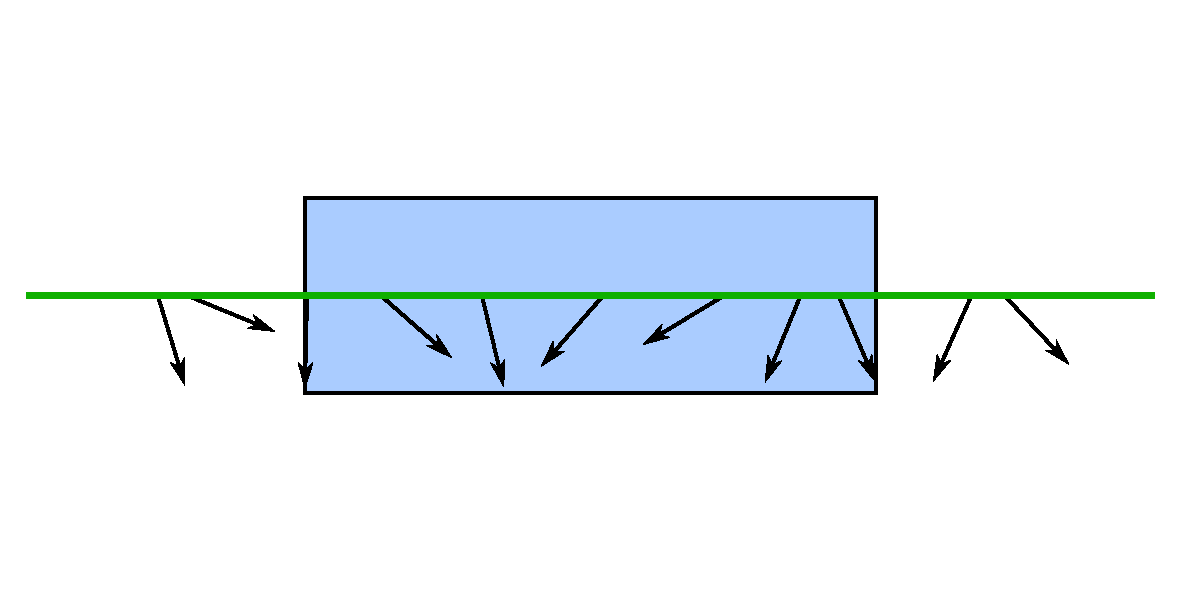
\includegraphics[width=0.48\textwidth]{images/CosmicGammaBackground/CRYHitbox1.pdf}
        \label{fig:CRYHitbox1}
    }
    \subfloat[CRY Hitbox b][]
    {
        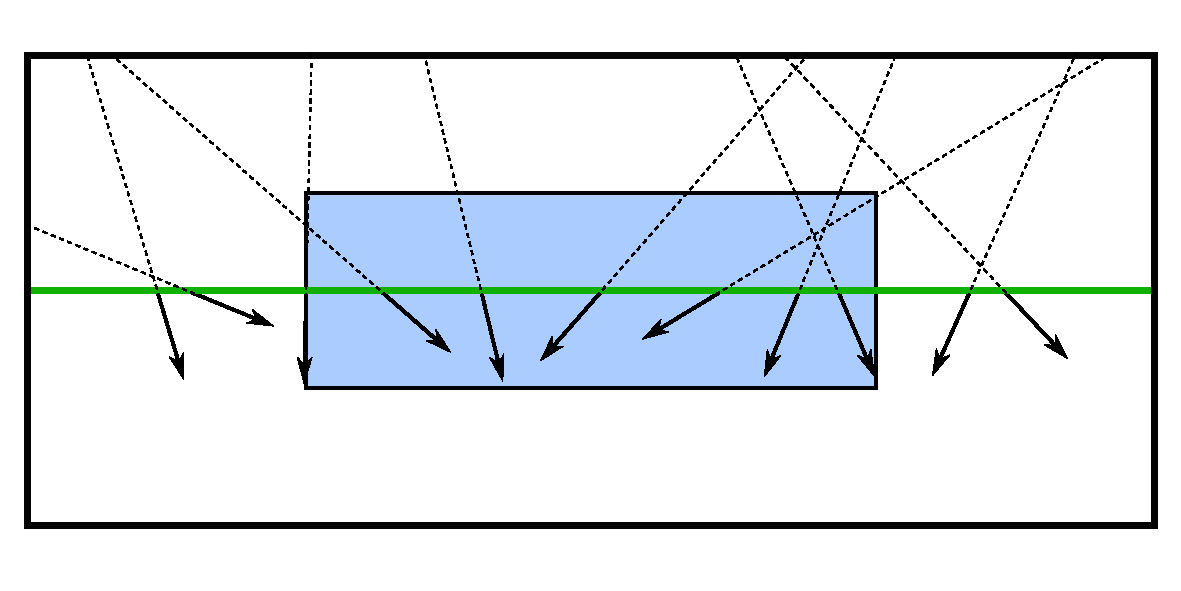
\includegraphics[width=0.48\textwidth]{images/CosmicGammaBackground/CRYHitbox2.pdf}
        \label{fig:CRYHitbox2}
    }
    \\
    \subfloat[CRY Hitbox c][]
    {
        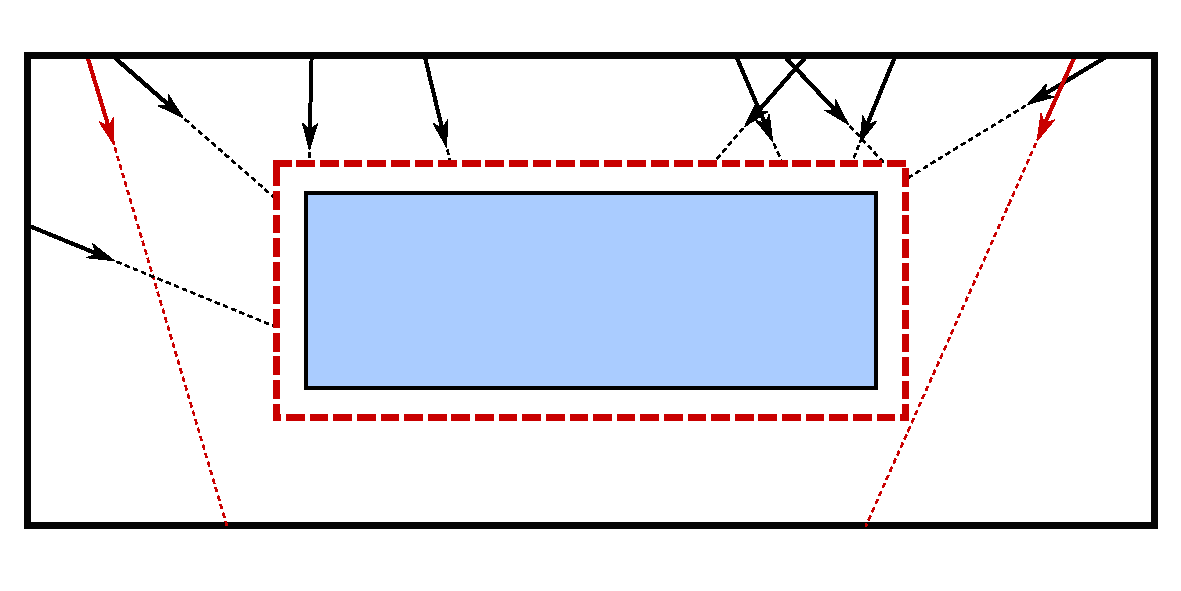
\includegraphics[width=0.48\textwidth]{images/CosmicGammaBackground/CRYHitbox3.pdf}
        \label{fig:CRYHitbox3}
    }
    \subfloat[CRY Hitbox d][]
    {
        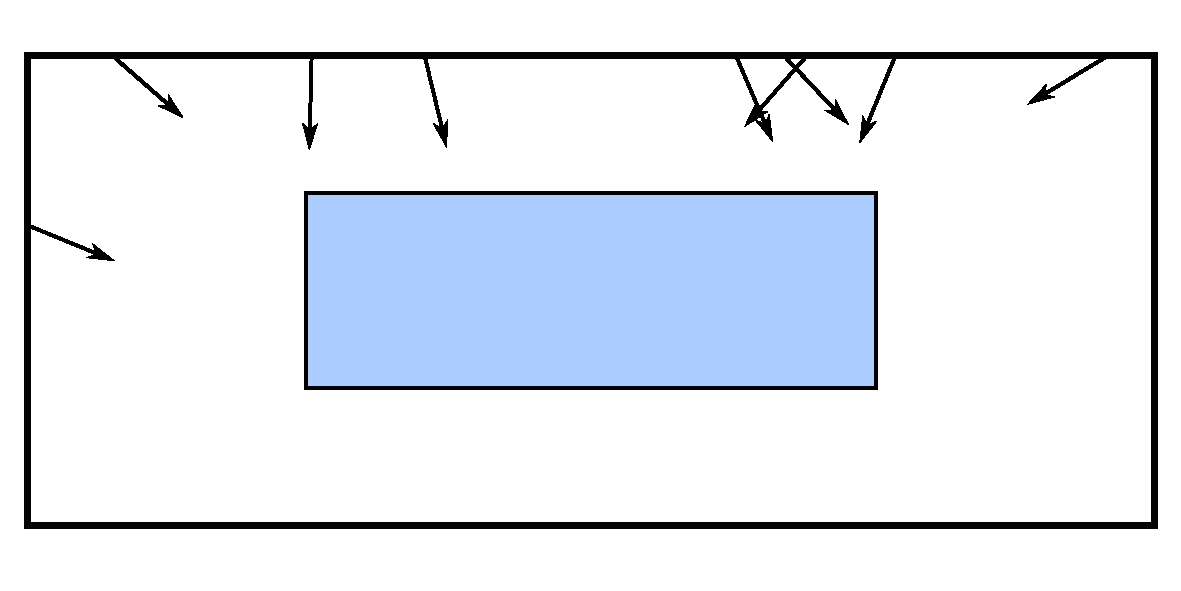
\includegraphics[width=0.48\textwidth]{images/CosmicGammaBackground/CRYHitbox4.pdf}
        \label{fig:CRYHitbox4}
    }
    \caption[2D Representation of the CRY Pre-Selection Algorithm]{This figure shows a \Gls{2d} representation of the CRY pre-selection algorithm. First, as shown in \subref{fig:CRYHitbox1}, the sub-box area of \gls{cry} (green) is placed in the centre of the active volume (light blue) and primary photons are generated, indicated by their unit momentum vectors (black). Thereafter, in \subref{fig:CRYHitbox2}, their positions are shifted to the edge of the simulations world-box, in the opposite direction of their momentum. Then, in \subref{fig:CRYHitbox3}, it is checked if the particle's trajectory intersects with a hit-box surrounding the detector (red dashed line). Finally, in \subref{fig:CRYHitbox4}, all particles missing said hit-box, are deleted and the \gls{geant} part of the simulation starts.}
    \label{fig:CRYHitbox}
\end{figure}

From here, \gls{geant}'s main task begins, simulating the passage of particles through the geometry while tracking their position, momentum, energy, and time. For this purpose, the above described, simplified detector geometry is defined in \gls{gdml} code \cite{GDML} and then feed into \gls{geant}. For the tracking part a so-called physics list needs to be defined, containing all physics processes simulated. Since I only consider photons as primary particles, the list is reduced to only photons, electrons, positrons and their respective electromagnetic interactions. All these simulated processes and the corresponding primary and secondary particles are listed in table \ref{tab:G4PhysicsList}. Furthermore, \gls{geant} only tracks particles until they fall below an energy threshold, in order to safe computing time. For this work I chose the standard energy threshold of $E \geq \SI{0.1}{\electronvolt}$.
\begin{table}[hbtp]
	\centering
    \caption[Geant4 Physics List Settings]{\Gls{geant} physics list settings of photons $\gamma$, electrons $e^-$, and positrons $e^+$. The simulated processes only contain electro magnetic interactions.}
    \label{tab:G4PhysicsList}
	\begin{tabu}{cll}
        \toprule
        Simulated Particle & Physics Process & Geant4 Label \\
        \midrule
        \multirow{3}{*}{$\gamma$} & Photoelectric effect & G4PhotoElectricEffect\\
                                  & Compton scattering & G4ComptonScattering \\
                                  & Pair production (conversion) & G4GammaConversion \\
        \midrule
        \multirow{3}{*}{$e^-$}    & Multiple scattering & G4eMultipleScattering \\
                                  & Ionisation & G4eIonisation \\
                                  & Bremsstrahlung & G4eBremsstrahlung \\
        \midrule
        \multirow{4}{*}{$e^+$}    & Multiple scattering & G4eMultipleScattering  \\
                                  & Ionisation & G4eIonisation \\
                                  & Bremsstrahlung & G4eBremsstrahlung \\
                                  & Annihilation & G4eplusAnnihilation \\
        \bottomrule
    \end{tabu}
\end{table}
\Gls{geant} offers access to the simulation through several classes called user actions. For instance all operations the user wants to perform at the start or the end of a simulation run, are executed through the user run action called ``G4UserRunAction''. I use this class to initialise the data container at the start of the run and write the data to a file at the end. A \gls{geant} simulation is a stepped process, meaning every interaction of a particle happens at a step point in space and time. How long these steps are and which interactions occur at the step points, is determined by a set of tuned random number generators, hence the name \acrfull{mc}. The software offers access to all information at such a step point through the user stepping action class ``G4UserSteppingAction''. This class is used to extract all the relevant information of the primary, and some secondary particles. The primary photon is tracked in order to determine if it interacts with the active volume. Once it enters the active volume its current position $\vec{x}_\gamma$, kinetic energy $E_\gamma$, and momentum direction $\hat{p}_\gamma$ are registered. If it interacts through the photoelectric effect or Compton scattering, the same data variables are stored right at the interaction \gls{Vertex} of the photon. But this time it is the information of the secondary electron, \ie $\vec{x}_e$, $E_e$, and $\hat{p}_e$. Pair production is not tracked, for it does not correspond to the $\nu_e$ background signature of a single electron, although some misidentification could still occur. The process has to be simulated regardless, because its absence would contribute to an increase in the other two photon related processes (see table \ref{tab:G4PhysicsList}). The information is then stored in memory in my own data class until the end of the run, when it is written into a file. This leads to a potential memory leak when computing too many events, but it also reduces costly read-write cycles and thus increases performance substantially.

One thing that \gls{geant} is not able to simulate is the charge carrier drift in the active volume. Since most of the cosmic-ray gamma events occur outside of the \gls{BeamGate}, the phenomenon of drifted in cosmic pileup events in \glspl{lartpc} plays a major role here (see section \ref{sec:CosmicPileup}). Therefore drift is simulated in the data analysis code, \ie post-simulation. I assume that the cosmic flux is uniformly distributed through time, which also results in an uniform distribution on the drift axis ($x$-coordinate). Thus a random number generator is used to give every stored electron a new $x$-position, while the $y$- and $z$-coordinates remain unchanged. Furthermore, several cuts are applied after the drift simulation, in order to quantify the background level. Finally ROOT is used to create various distributions, draw graphs, and handle statistics. The results of above-described simulations will be shown and discussed in the following sections in two parts. First I will investigate the raw \gls{cry} output, comparing it to measurements and theories, and second I will present the results of the full simulation including various selections.

Before we can start with the results, we need to introduce the two coordinate systems used in this work. In the first part of the results, we will use the standard coordinate system as used in astroparticle physiscs with a $z$-axis vertical, and the $y$- and $x$-axis horizontal to the earths surface. In this coordinate system two angles are defined: the azimuth angle, $\phi^{\prime}$, and the zenith angle, $\theta^{\prime}$. The azimuth angle is defined in the $x$-$y$-plane in the interval $-\pi \leq \phi^{\prime} \leq \pi$, with $\phi^\prime = 0$ on the $x$-axis and $\phi^\prime = \pi/2$ on the $y$-axis. The zenith angle is defined from the $z$-axis, where $\theta^\prime = 0$, to the $x$-$y$-plane, where $\theta^\prime = \pi/2$. Hence, the standard system covers only a hemisphere. The MicroBooNE coordinate system, on the other hand, is rotated around the $x$-axis by \SI{90}{\degree} and thus exhibits a horizontal $x$-$z$-plane and $y$ as the vertical axis (see section \ref{sec:MicroBooNEDetector}, especially figure \ref{fig:MicroBooNECoordinateSystem}). Relative to the three axis, the angles $\phi$ and $\theta$ of the MicroBooNE system are defined the same way as $\phi^{\prime}$ and $\theta^{\prime}$. In MicroBooNE the $\theta$-angle is defined in the interval $0 \geq \theta \geq \pi$, thus covering a full sphere, instead of a hemisphere. Another difference of the two systems is the point of reference. The reference of the standard system is the observer, \ie $\phi^\prime$ and $\theta^\prime$ constitute the angles where the particle is originating from, while the reference in the MicroBooNE system is the particle itself and thus $\phi$ and $\theta$ directly show the direction of the particle's momentum. In the following the angles of both systems are treated as equals as they share very same properties.

The only directional information \gls{cry} and \gls{geant} provide, is the unit momentum vector $\hat{p} = (p_x,p_y,p_z)$. Hence, these angles first need to be extracted from $\hat{p}$. The $\theta$-angle is quite simple to calculate, since the vertical component of the momentum vector is just the cosine of said angle, $p_z = \cos{(\theta)}$. In order to determine the $\phi$-angle, $\hat{p}$ has to be rotated onto the $x$-$y$-plane which gives us a new unit vector $\hat{p}^{\prime} = (p_{x}^{\prime},p_{y}^{\prime},0)$. From this we are able to derive $p_{x}^{\prime} = \cos{(\phi)}$ and $p_{y}^{\prime} = \sin{(\phi)}$. When assuming the angle space as $-\pi \leq \phi \leq \pi$, we get,
\begin{align} \label{eq:AngleCalculation}
        \phi &= \sgn (p_{y}^{\prime}) \arccos{(p_{x}^{\prime})}, \nonumber \\
        \theta &= \arccos{\left(p_z\right)}.
\end{align}
Above calculations are valid for both, the MicroBooNE's coordinate system with $\phi$ and $\theta$ as well as the standard coordinate system with $\phi^\prime$ and $\theta^\prime$. The angle calculations described in this paragraph are visualised in figure \ref{fig:AngleCalculation}.
\begin{figure}[htbp]
    \centering
    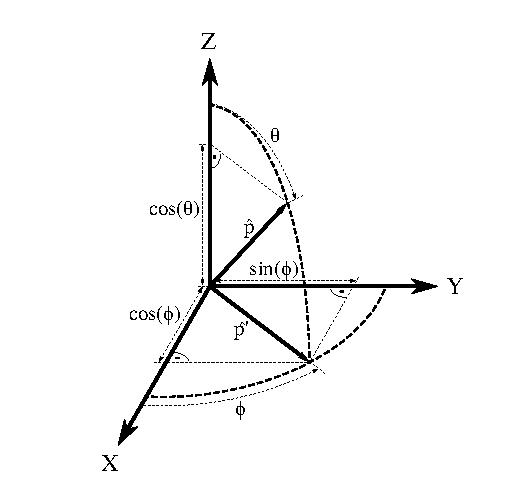
\includegraphics[width=0.7\textwidth]{images/CosmicGammaBackground/AngleCalculation.pdf}
    \caption[Angle Calculation from a Unit Momentum Vector]{This figure visualises the procedure of extracting the angles $\phi^{(\prime)}$ and $\theta^{(\prime)}$ from a unit momentum vector $\hat{p}$ as formulated in equation \ref{eq:AngleCalculation}.}
    \label{fig:AngleCalculation}
\end{figure}

%-----------------------------------------------------------------------------------------------------------------------------------------------------------------
\section{Raw CRY Output Results} \label{sec:CRYAnalysis}
Before simulating the background rates in MicroBooNE, I first investigated the raw \gls{cry} photon output. On that account I generated one million correlated cosmic-ray showers, while considering only photons. The \gls{cry} settings used were the same as listed in table \ref{tab:CRYSettings}, resulting in the output listed in table \ref{tab:CRYResults} below.
\begin{table}[hbtp]
	\centering
    \caption[Raw CRY Cosmic-Ray Photon Output]{Raw \gls{cry} cosmic-ray photon output by one million correlated cosmic-ray showers generated on a $\SI{100}{\metre} \times \SI{100}{\metre}$ plane.}
    \label{tab:CRYResults}
	\begin{tabu}{llrl}
        \toprule
        Output variable & Symbol & Value & Unit \\
        \midrule
        Generated showers & $N_\text{gen}$ & \num{1000000} & \\
        Generated photons & $N_\gamma$ & \num{1261511} & \\
        Time simulated & $T$ & \num{0.774}& \si{\second} \\
        Photon flux & $\Phi_\gamma$ & \num{0.0163} & \si{\per\centi\metre\per\second} \\
        Min. kinetic Energy & $E_{\text{min}}$ & \num{1} & \si{\mega\electronvolt} \\
        \bottomrule
    \end{tabu}
\end{table}

Now, let us look at some noteworthy distributions of the raw \gls{cry} output, starting with the directional intensity $I_\gamma(\phi^{\prime},\theta^{\prime})$ as defined by equation \ref{eq:DirectionalIntensity} in section \ref{sec:CosmicRayTheory}. Since I am only interested in a \gls{1d} view of the directional intensity, \ie $I_\gamma(\phi^{\prime})$ and $I_\gamma(\theta^{\prime})$, and the fact that I am facing a binned function, equation \ref{eq:DirectionalIntensity} has to be adapted. First of all, every differential that is not a binned entity has to be integrated, \eg $\int_0^A dA^{\prime} = A$ or $\int_0^T dt^{\prime} = T$, where in this case $A$ is CRY's ``sub-box'' area and $T$ the simulated time period. When looking at $I_\gamma(\phi^{\prime})$ and $I_\gamma(\theta^{\prime})$ the respective angular differentials, $d\phi^{\prime}$ or $d\theta^{\prime}$, become the bin width $\delta\phi^{\prime}$ or $\delta\theta^{\prime}$. The respective other differential is also integrated over its angle space. Furthermore, the control variables $\phi^{\prime}$ and $\theta^{\prime}$ are no longer continuous, but discrete values of a bin with the number $n$, \ie $\phi^{\prime}_n$ and $\theta^{\prime}_n$, respectively. Thus I arrive at the two formulas
\begin{align}\label{eq:BinnedDirectionalIntensityPhi}
    I_\gamma(\phi^{\prime}_n) &= \frac{\delta N_\gamma(\phi^{\prime}_n)}{AT \, \delta\phi^{\prime} \int_{0}^{\frac{\pi}{2}}d\theta^{\prime}\sin{(\theta^{\prime})}} =\frac{\delta N_\gamma(\phi^{\prime}_n)}{AT \, \delta\phi^{\prime}}, \\[5pt]
    I_\gamma(\theta^{\prime}_n) &= \frac{\delta N_\gamma(\theta^{\prime}_n)}{AT\, \delta \theta^{\prime}\sin{(\theta^{\prime}_n)} \int_{-\pi}^{+\pi}d\phi^{\prime}} = \frac{\delta N_\gamma(\theta^{\prime}_n)}{2\pi AT\, \delta\theta^{\prime}\sin{(\theta^{\prime}_n)}},
    \label{eq:BinnedDirectionalIntensityTheta}
\end{align}
whereby $\delta N_\gamma(\phi^{\prime}_n)$ denotes the number of photons registered in a single bin with value $\phi^{\prime}_n$ and $I_\gamma(\phi^{\prime}_n)$ the resulting directional Intensity of said bin. Dividing $\delta N_\gamma(\phi^{\prime}_n)$ by the bin width, in this case $\delta\phi^{\prime}$, also ensures a bin-size independent graph. Furthermore, the calculation of $I_\gamma(\theta^{\prime}_n)$ in equation \ref{eq:BinnedDirectionalIntensityTheta} indicates that each bin entry needs to be scaled by the inverse of the sine of the bin's zenith angle, $1/\sin{(\theta^{\prime}_n)}$, in order to achieve solid angle dependency of $I_\gamma(\theta^{\prime}_n)$. The results of the raw \gls{cry} output after applying above calculations are shown in figure \ref{fig:CRYDirectionalIntensity}.
\begin{figure}[htbp]
    \centering
    % This operation here maxes the two plots the same height, by still providing full text width
    \subfloat[Raw CRY Photon Azimuth Angle Intensity][]
    {
        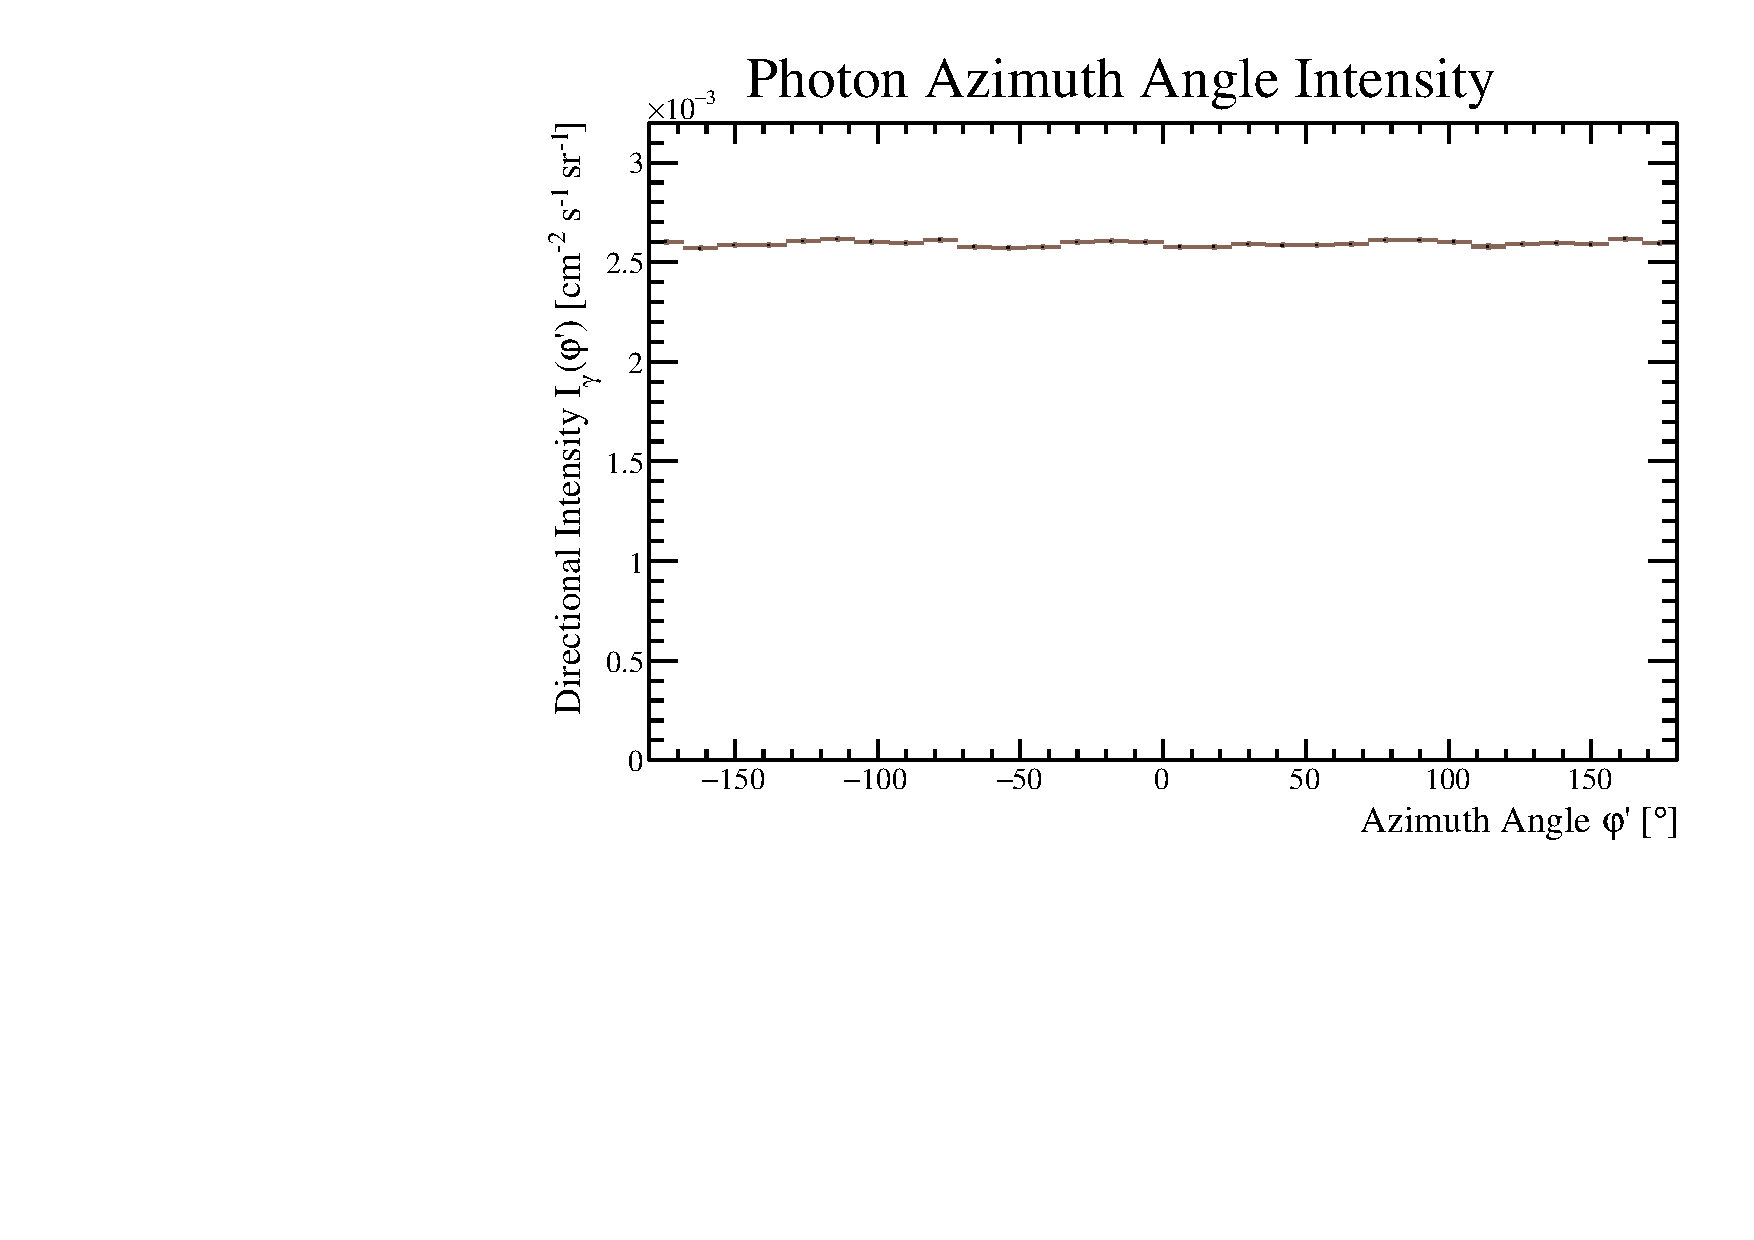
\includegraphics[width=0.48\textwidth]{images/CosmicGammaBackground/CRYPhi.pdf}
        \label{fig:CRYDirectionalIntensityPhi}
    } %\qquad
    \subfloat[Raw CRY Photon Zenith Angle Intensity][]
    {
        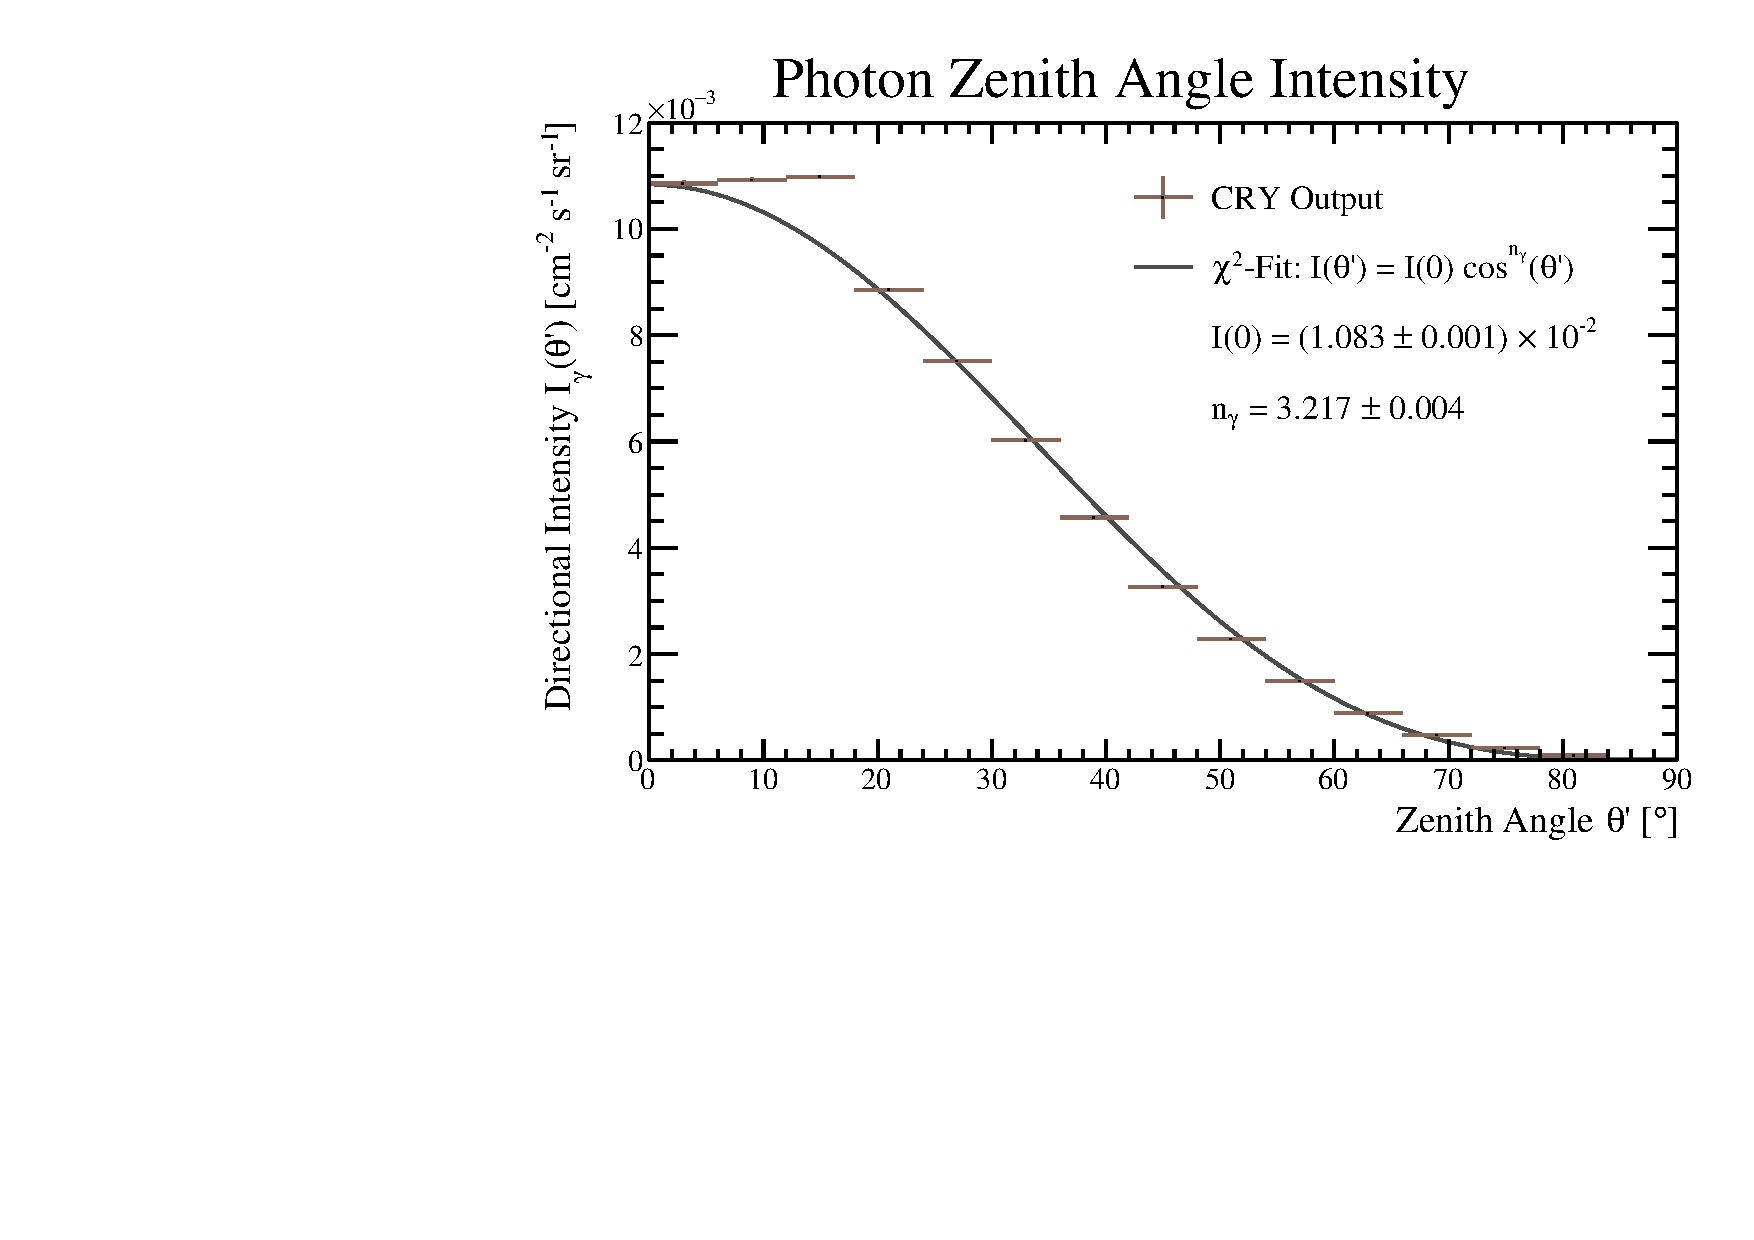
\includegraphics[width=0.48\textwidth]{images/CosmicGammaBackground/CRYTheta.pdf}
        \label{fig:CRYDirectionalIntensityTheta}
    }
    \caption[Raw Cosmic-Ray Photon Directional Intensity Provided by CRY]{These figures show the raw cosmic-ray photon directional intensity $I_\gamma$ provided by \gls{cry}. \subref{fig:CRYDirectionalIntensityPhi} depicts the directional intensity as a function of the azimuth angle, $I_\gamma(\phi^{\prime})$, calculated according to equation \ref{eq:BinnedDirectionalIntensityPhi}. \subref{fig:CRYDirectionalIntensityTheta} shows the directional intensity as a function of the zenith angle, $I_\gamma(\theta^{\prime})$, in accordance to equation \ref{eq:BinnedDirectionalIntensityTheta}. Additionally, I performed a $\chi^2$-fit of the $\theta^\prime$ dependent directional intensity $I_\gamma(\theta^\prime) = I_\gamma(\SI{0}{\degree}) \cos^{n_{\gamma}}{(\theta^\prime)}$ introduced in equation \ref{eq:ThetaDependentIntensity}. The fit parameters were $I_\gamma(\theta^{\prime}=\SI{0}{\degree})$ and $n_\gamma$. In both graphs the units of the $X$-axis are converted from radian into degrees, for better readability.}
    \label{fig:CRYDirectionalIntensity}
\end{figure}
As can be seen, the $I_\gamma(\phi^{\prime})$ distribution is flat over all $\phi^{\prime}$-angles. This is expected and acts as a sanity check of this simulation. $I_\gamma(\theta^{\prime})$ features a plateau between \SIrange{0}{20}{\degree}, and a $\cos^{n_\gamma}{(\theta^{\prime})}$ shaped decline thereafter, with zero intensity at $\theta^{\prime} = \SI{90}{\degree}$. Said behaviour is also expected, since incident cosmic-rays at higher zenith angles have to cross ever increasing distances through the atmosphere, resulting in higher energy losses of these showers. Furthermore, I performed a $\chi^2$-fit, using the function $I_\gamma(\theta^\prime) = I_\gamma(\SI{0}{\degree}) \cos^{n_{\gamma}}{(\theta^\prime)}$ introduced in equation \ref{eq:ThetaDependentIntensity}, with the free parameters being $I_\gamma(\SI{0}{\degree}) = \SI{1.083(1)e-2}{\per\centi\metre\squared\per\second\per\steradian}$ and $n_\gamma = \num{3.217(4)}$. With the fitted function drawn on top of the \gls{cry} output, it becomes obvious, that \gls{cry} produces a slight photon excess around $\theta^\prime = \SI{10}{\degree}$, where $I_\gamma(\theta^{\prime})$ does not follow a $\cos^{n_\gamma}{(\theta^{\prime})}$ distribution. I consciously decided against showing the \gls{2d} $I_\gamma(\phi^{\prime},\theta^{\prime})$ graph, as it remains featureless on the $\phi^{\prime}$-axis and would thus not show more information than already provided by the two graphs above.

The next observable I would like to present, is \gls{cry}'s photon differential energy spectrum, $j_\gamma(E)$. I also introduced said observable in section \ref{sec:CosmicRayTheory}. Here I take the same approach as before with $I_\gamma$ and transform the continuous function of $j_\gamma(E)$ from equation \ref{eq:DifferentialEnergySpectrum}, into a binned one, \ie $j_\gamma(E) \to j_\gamma(E_n)$. Thereby the differentials $dA$, $dt$, and $d\Omega^{\prime}$ have to be integrated over their respective spaces, as the $j_\gamma(E)$ exhibits only an energy dependence. Because the energy spectrum ranges over a large interval in both $E$ and $j_\gamma(E)$, it is usually represented in a log-log graph. Now, if the bins are to remain in a visually equally spaced manner on the logarithmic axis, the bin width $\delta E$ becomes variable, \ie a function of bin energy $\delta E(E_n)$ or $\delta E_n$ in short with $\delta E_n \propto 10^{E_n}$. Thus I deduce the single bin function as
\begin{equation} \label{eq:BinnedDifferentialEnergySpectrum}
    j_\gamma(E_n) = \frac{\delta N_\gamma(E_n)}{2\pi AT\, \delta E_n}.
\end{equation}
The differential energy spectrum of simulated cosmic-ray photons provided by \gls{cry} is shown in figure \ref{fig:CRYKineticEnergy}.
\begin{figure}[htbp]
    \centering
    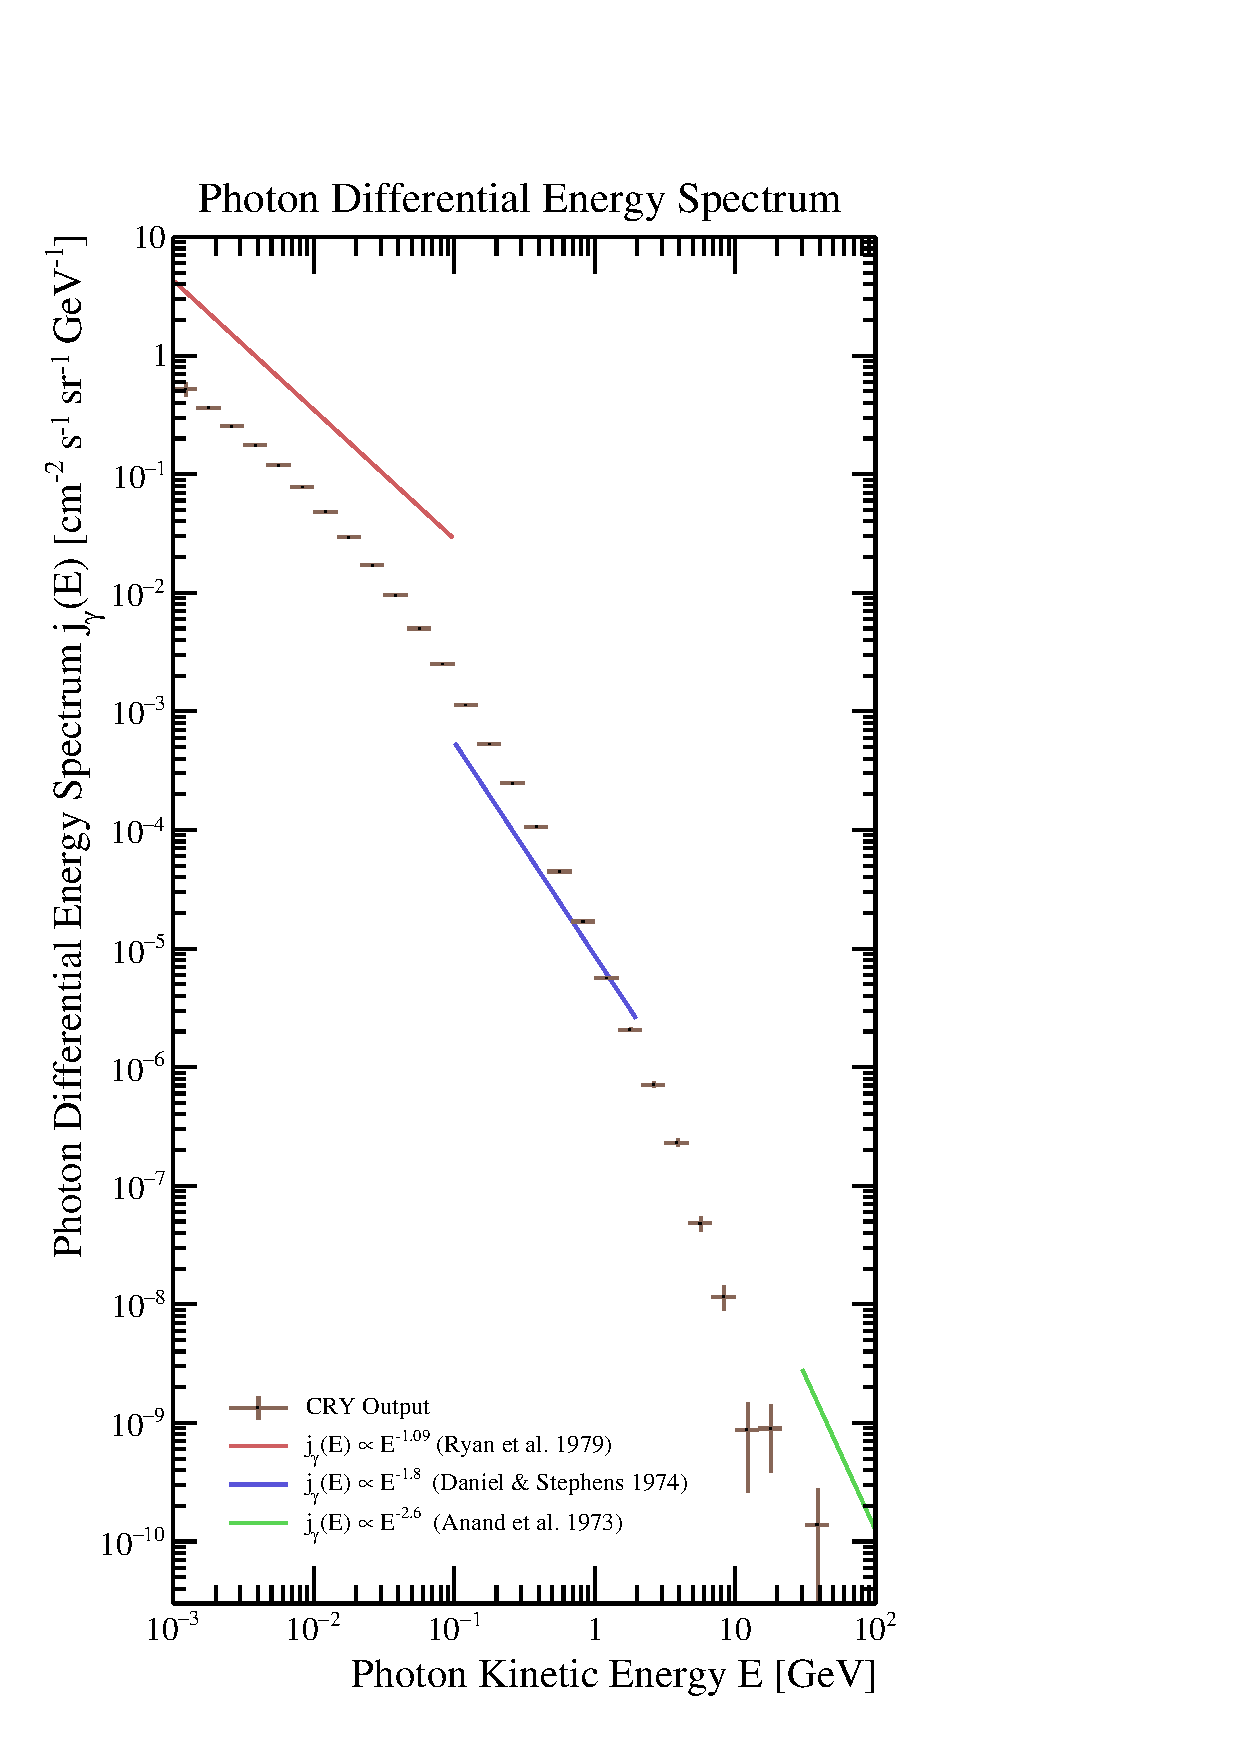
\includegraphics[width=0.8\textwidth]{images/CosmicGammaBackground/CRYKineticEnergy.pdf}
    \caption[Raw Cosmic-Ray Photon Differential Energy Spectrum Provided by CRY]{This figure shows the raw cosmic-ray photon differential energy spectrum, $j_\gamma(E)$, as provided by \gls{cry}. The \gls{cry} output, in brown, was calculated according to equation \ref{eq:BinnedDifferentialEnergySpectrum}. For comparison, three power law fits, based on cosmic-ray photon measurements, are drawn in different colours. Represented in red, for $E \leq \SI{0.1}{\giga\electronvolt}$, is the fit of Ryan \etal (1979) \cite{CosmicGammaSpectrumFit1}, with $j_\gamma(E) \propto E^{-1.09}$. The result of Daniel and Stephens (1974) \cite{CosmicGammaSpectrumFit2}, with $j_\gamma(E) \propto E^{-1.8}$ for energies $\SI{0.1}{\giga\electronvolt} \leq E \leq \SI{2}{\giga\electronvolt}$, is drawn in blue. Illustrated in green is the best fit of Anand \etal (1973) \cite{CosmicGammaSpectrumFit3} with $j_\gamma(E) \propto E^{-2.6}$ for $\SI{30}{\giga\electronvolt} \leq E$. The latter two functions were fitted on high altitude data and are scaled, in order to ensure compatibility with the sea-level output of \gls{cry}.}
    \label{fig:CRYKineticEnergy}
\end{figure}
Moreover, I added fits from three different cosmic photon measurements to the graph. All three experiments used the power law function for the differential energy spectrum $j(E) = AE^{-\gamma}$ introduced in equation \ref{eq:CosmicRayEnergyDependency}. Said measurements are:
\begin{enumerate}
    \item Ryan \etal (1979) \cite{CosmicGammaSpectrumFit1}: with an energy range of $\SI{1}{\mega\electronvolt} \leq E \leq \SI{0.1}{\giga\electronvolt}$, vertical depth of $X_1 = \SI{1000}{\gram\per\centi\metre\squared}$, they found $j_\gamma(E) = \num{2.3e-3}E^{-1.09}$.
    \item Daniel and Stephens (1974) \cite{CosmicGammaSpectrumFit2}: with an energy range of $\SI{0.1}{\giga\electronvolt} \leq E \leq \SI{2}{\giga\electronvolt}$, vertical depth of $X_1 = \SI{10}{\gram\per\centi\metre\squared}$, they found $j_\gamma(E) = \num{1.3e-3}E^{-1.8}$.
    \item Anand \etal (1973) \cite{CosmicGammaSpectrumFit3}: with an energy range of $\SI{30}{\giga\electronvolt} \leq E \leq \SI{1}{\tera\electronvolt}$, vertical depth of $X_1 = \SI{14.3}{\gram\per\centi\metre\squared}$, they found $j_\gamma(E) = \num{1.14e-2}E^{-2.6}$.
\end{enumerate}
All graphs in figure \ref{fig:CRYKineticEnergy} are scaled, in order to accept input energies in units of $[\si{\giga\electronvolt}]$ and to output $j(E)$ in units of $[\si{\per\centi\metre\squared\per\second\per\steradian\per\giga\electronvolt}]$. As indicated above, the latter two measurements feature low vertical depths, which I first had to correct before overlaying them with \gls{cry}'s differential energy spectrum. Thus I employed the height dependency formula from equation \ref{eq:CosmicRayEnergyDependency}, to scale $j_\gamma(E)$ by $\exp(-(X_2-X_1)/\Lambda)$ for $X_2 = \SI{1000}{\gram\per\centi\metre\squared}$. Using the energy dependence of $\Lambda$ from \cite{CosmicGammaSpectrumFit2}: I scaled the 2\textsuperscript{nd} fit function with $\Lambda = \SI{185}{\gram\per\centi\metre\squared}$, and the 3\textsuperscript{rd} using $\Lambda = \SI{155}{\gram\per\centi\metre\squared}$.

Since the height dependency formula should in principle only be used for hadrons, the placing of the corrected fit lines might well be off and has to be taken with a grain of salt. Still there might be some validity, as photons with higher energy originate mainly from the hadronic component of cosmic-ray showers. Furthermore, the power law part of the functions is expected to be valid no matter the elevation. As can be seen in figure \ref{fig:CRYKineticEnergy}, \gls{cry}'s energy spectrum seems to fit the slopes of the measured curves quite nicely, although they exhibit quite large offsets at certain energies. However, I generally think that power law fits are not reflecting reality below \SI{1}{\giga\electronvolt}, as the real measurement points curve away from the fit lines in all publication I reviewed for this work. This becomes obvious when considering the publications of the three measurements cited here, and the great collection of spectra in Grieder's book \cite{CosmicRayGrieder}. \Gls{cry} shows a similar curve at low energies as the data points in the publications. Keep in mind, that \gls{cry}'s photon output is purely based on \gls{mc} simulation, with all the weirdness which can come with it. Therefore it is advisable to double check these outputs with real data, as I did here.

Next, I investigate the integral energy spectrum of the photons generated by \gls{cry}, $J_\gamma(E)$, introduced in equation \ref{eq:IntegralEnergySpectrum}. It is defined as the integral of $j_\gamma(E^{\prime})\, dE^\prime$, between $E$ and $\infty$. As I am calculating $J_\gamma(E)$ in a binned histogram, said integral becomes a sum of all the bins with an energy higher than $E$ multiplied by their respective energy bin width. Since there are no histograms with an infinite number of bins, $\infty$ as an upper bound is replaced with the maximum bin number $n_\text{max}$. For a bin with the number $n$ we thus get:
\begin{equation} \label{eq:BinnedIntegralEnergySpectrum}
    J_\gamma(E_n) = \sum_{i=n}^{n_\text{max}} j_\gamma(E_i) \delta E_i = \frac{1}{2\pi AT} \sum_{i=n}^{n_\text{max}} \delta N_\gamma(E_i).
\end{equation}
The raw integral photon energy spectrum produced by \gls{cry} is shown in figure \ref{fig:CRYIntegratedEnergy}.
\begin{figure}[htbp]
    \centering
    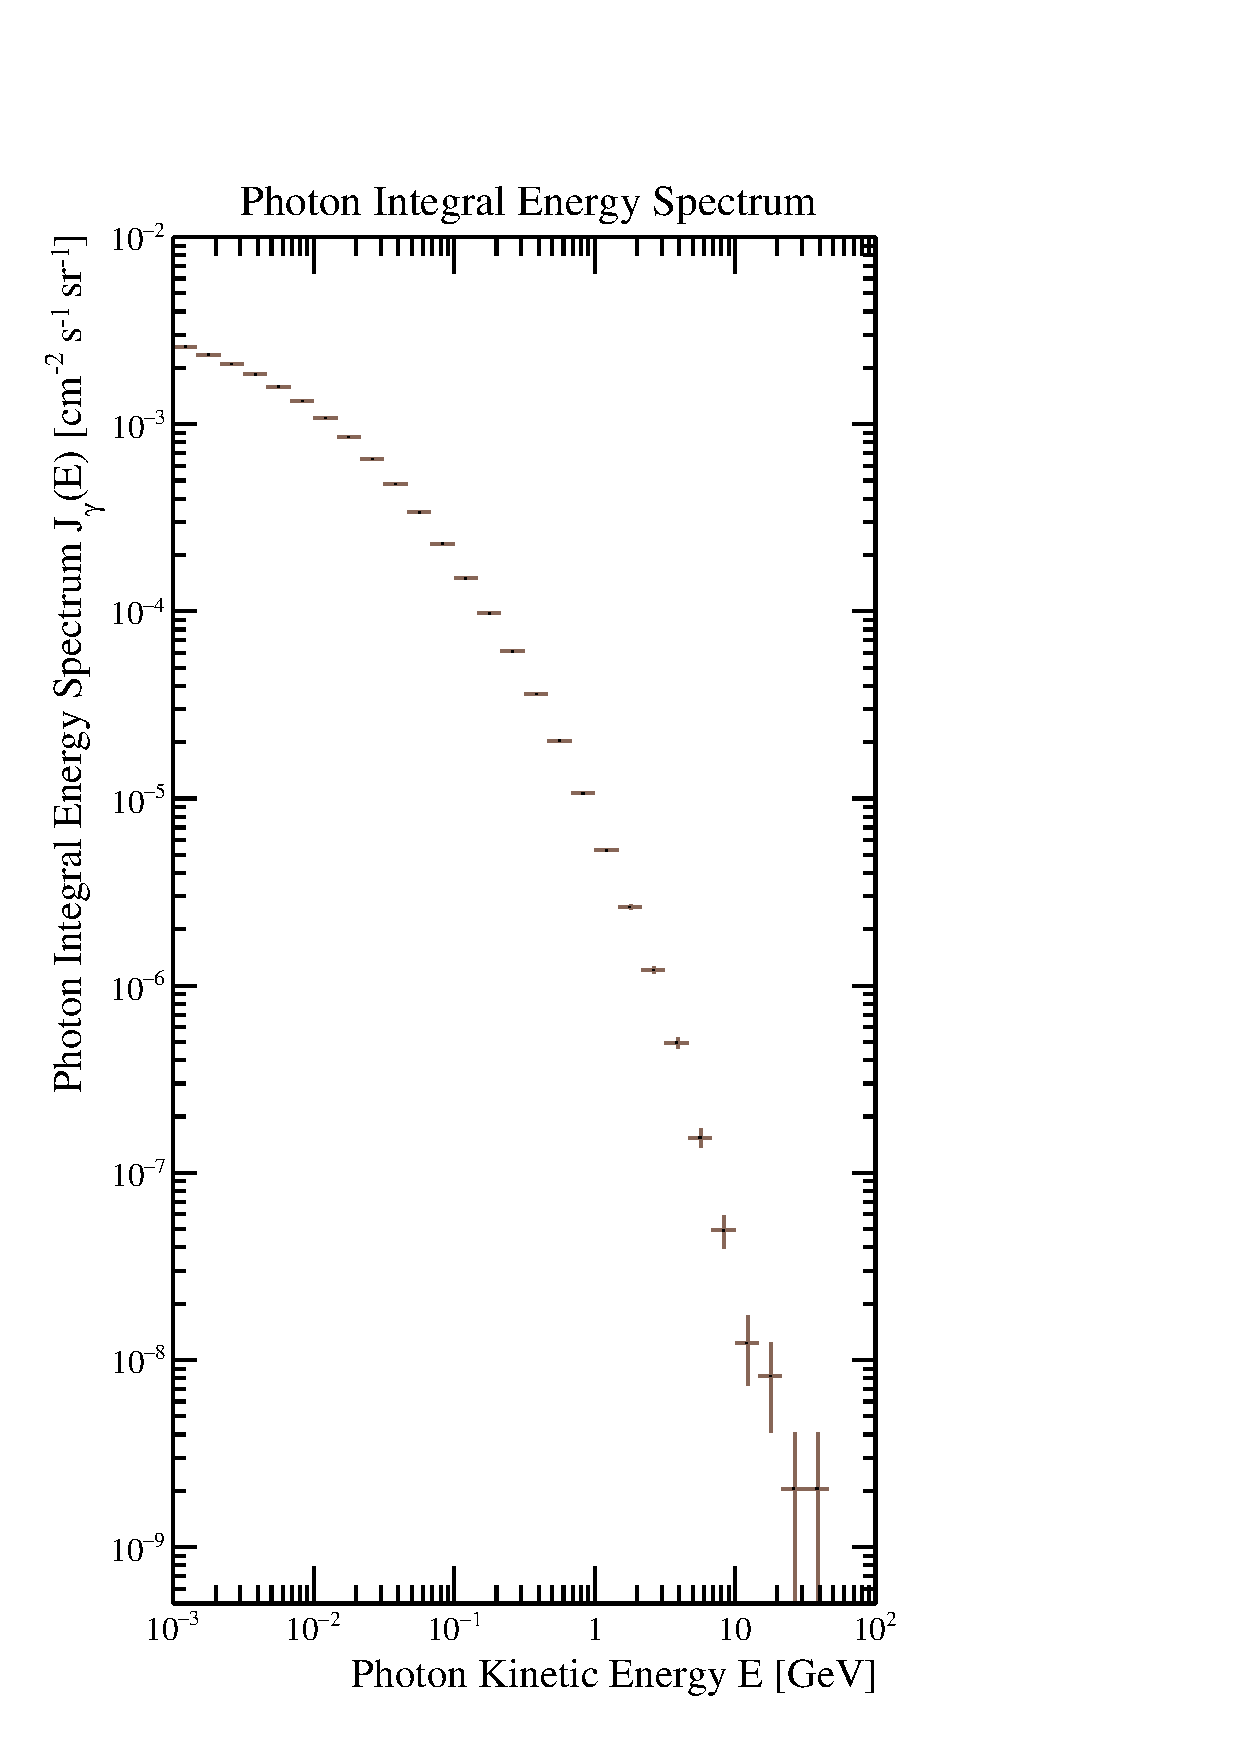
\includegraphics[width=0.8\textwidth]{images/CosmicGammaBackground/CRYIntegratedEnergy.pdf}
    \caption[Raw Cosmic-Ray Photon Integral Energy Spectrum Provided by CRY]{Depicted above is the raw cosmic-ray photon integral energy spectrum, $J_\gamma(E)$, provided by \gls{cry}. The bin entries were calculated according to equation \ref{eq:BinnedIntegralEnergySpectrum}.}
    \label{fig:CRYIntegratedEnergy}
\end{figure}
This kind of integrated spectrum is very useful for background considerations, since each bin shows the expected number of background events with energies higher or equal than a respective threshold. This threshold energy is usually given by the detector's sensitivity. 

Here ends the analysis of the generated cosmic-ray photons generated by \gls{cry}. Apart from some \gls{mc} weirdness in the zenith angle dependent directional intensity (see figure \ref{fig:CRYDirectionalIntensityTheta}), which could be a binning artefact, the gammas produced seem to be reflecting reality quite well. 

%-----------------------------------------------------------------------------------------------------------------------------------------------------------------
\section{Cosmic Gamma-Ray Background in MicroBooNE}
As stated before, the goal of this study is to estimate the cosmic photon background for the \gls{lee} in MicroBooNE. But, before considering the background, I would like to introduce the signal said background is interfering with. If we were to apply the \gls{lee} found by MiniBooNE to the MicroBooNE detector we would find an event rate of \num{48.5} per \num{e20} \gls{pot} in the active volume. The \gls{bnb} delivers \num{5e12} \gls{pot} per beam pulse \cite{BNBBeamFlux} which corresponds to \num{2.43e-6} expected \gls{lee} events in the active volume in one pulse. Since MicroBooNE uses a \gls{fv}, which I will introduce later, this result has to be scaled by the volume fraction. Hence, we get \num{1.91e-6} expected \gls{lee} events in the \gls{fv}, or $\sim\num{2e-6}$ as we are dealing with an estimate anyway. Since we have only one \gls{bnb} event per \gls{tpc} readout window, the same number applies in per readout window units. This number, $\sim\num{2e-6}$ per readout window, should be kept in mind in order to compare the background rates calculated in this section. MicroBooNE's operational \gls{tpc} readout window is \SI{2.25}{\milli\second} long meaning that, for every beam event, a cosmic background pileup is accumulated during this time frame.
% TODO cite the MicroBooNE LEE event number source (talk)?

For this simplified \gls{mc} simulation of the MicroBooNE active volume in a vacuum, a second sample of \gls{cry} photons was produced. This time, my code did not accept just any photon generated, but only those which fulfilled the hit-box requirements described above in section \ref{sec:SimulationSetup}. Hence, \gls{cry} was asked to produce a fixed number of photons and not correlated showers. Furthermore, I increased the sample size by a factor of five, compared to the \gls{cry} output analysis. As a reminder, the background signature investigated here is a single electron produced in the active volume by a cosmic-ray photon, \ie only photoelectric effect and Compton scattering is considered. This also leads to a change in nomenclature, with the \gls{cry} photons becoming the primary particles and their produced electrons the secondary particles. During the \gls{geant} part of the simulation, all \gls{Vertex} information about the single secondary electrons produced by the primary photon in MicroBooNE's active volume are stored. Later, the drift is simulated and the data analysed by a ROOT macro. A summary of the simulation output is listed in table \ref{tab:CosmicBackgroundResultsActive}. 
\begin{table}[hbtp]
	\centering
    \caption[Photon Induced Background Simulation Summary]{Simulation summary of the \gls{geant} photon induced background simulation.}
    \label{tab:CosmicBackgroundResultsActive}
	\begin{tabu}{llrl}
        \toprule
        Output variable & Symbol & Value & Unit \\
        \midrule
        Generated photons & $N_\text{gen}$ & \num{5000000} & \\
        Active volume hits & $N_\gamma$ & \num{2614216} & \\
        Produced single electrons & $N_e$ & \num{10145342} & \\
        Time simulated & $T$ & \num{473.4} & \si{\second} \\
        Photon hit rate & $r_\gamma$ & \num{5522} & \si{\per\second} \\
        Single electron production rate & $r_e$ & \num{21431} & \si{\per\second} \\
        Single $e^{-}$ Bgr. per readout frame (\SI{2.25}{\milli\second}) & & \num{48.2} & \\
        \bottomrule
    \end{tabu}
\end{table}

It can be seen that an average photon produces four single electrons before being absorbed or leaving the active volume again. Naturally, the MicroBooNE  collaboration applies several cuts in order to reduce the number of background events in the \gls{lee} studies. First there is always a \gls{fv} cut, which can vary between analysis groups of MicroBooNE. I decided to go with a cut of \SI{20}{\centi\metre} at the top, and \SI{10}{\centi\metre} at the sides as well as the bottom. In order to visualise the \gls{fv} cut, I used the differential volume rate defined in section \ref{sec:CosmicRayTheory}, equation \ref{eq:DifferentialVolumeRate}. As we are considering said distribution in two \gls{2d} views of the detector, the differential of the respective missing dimension has to be integrated. In addition, we can transfer the continuous function into a binned one suiting our needs, similar to the methods used during the \gls{cry} analysis before. This leaves us with the following two binned functions for the $(x,y)$ upstream view and $(z,y)$ side view:
\begin{align} \label{eq:BinnedDifferentialVolumeRateXY}
    \frac{dr_e(x_n,y_m)}{dV} = \frac{\delta N_e(x_n,y_m)}{T \, \delta x \, \delta y \, Z_{\text{TPC}}}, \\[5pt]
    \frac{dr_e(z_l,y_m)}{dV} = \frac{\delta N_e(z_l,y_m)}{T \, X_{\text{TPC}} \, \delta y \, \delta z}.
    \label{eq:BinnedDifferentialVolumeRateZY}
\end{align}
This time we use $e$ instead of $\gamma$ as the subscript of $r$, since we are considering electron rates. The indices $n$, $m$, and $l$ denote the bin number of the respective axis and $T$ again the time simulated. Furthermore, we have $\delta x$, $\delta y$, $\delta z$ defined as the bin widths, as well as the active volume dimensions $X_{\text{TPC}} = \SI{256.0}{\centi\metre}$ and $Z_{\text{TPC}} = \SI{1036.8}{\centi\metre}$ (see table \ref{tab:FieldCageDimensions}). Figure \ref{fig:GammaBackgroundDistribution} shows the single electron distribution within the active volume expressed as a differential volume rate in units of $[\si{\per\centi\metre\cubed\per\second}]$. The red box in said figure marks the contours of the \gls{fv}.   
\begin{figure}[htbp]
    \centering
    % This operation here maxes the two plots the same height, by still providing full text width
    \resizebox{\textwidth}{!}{
        \subfloat[Background Rate Side View][]
        {
            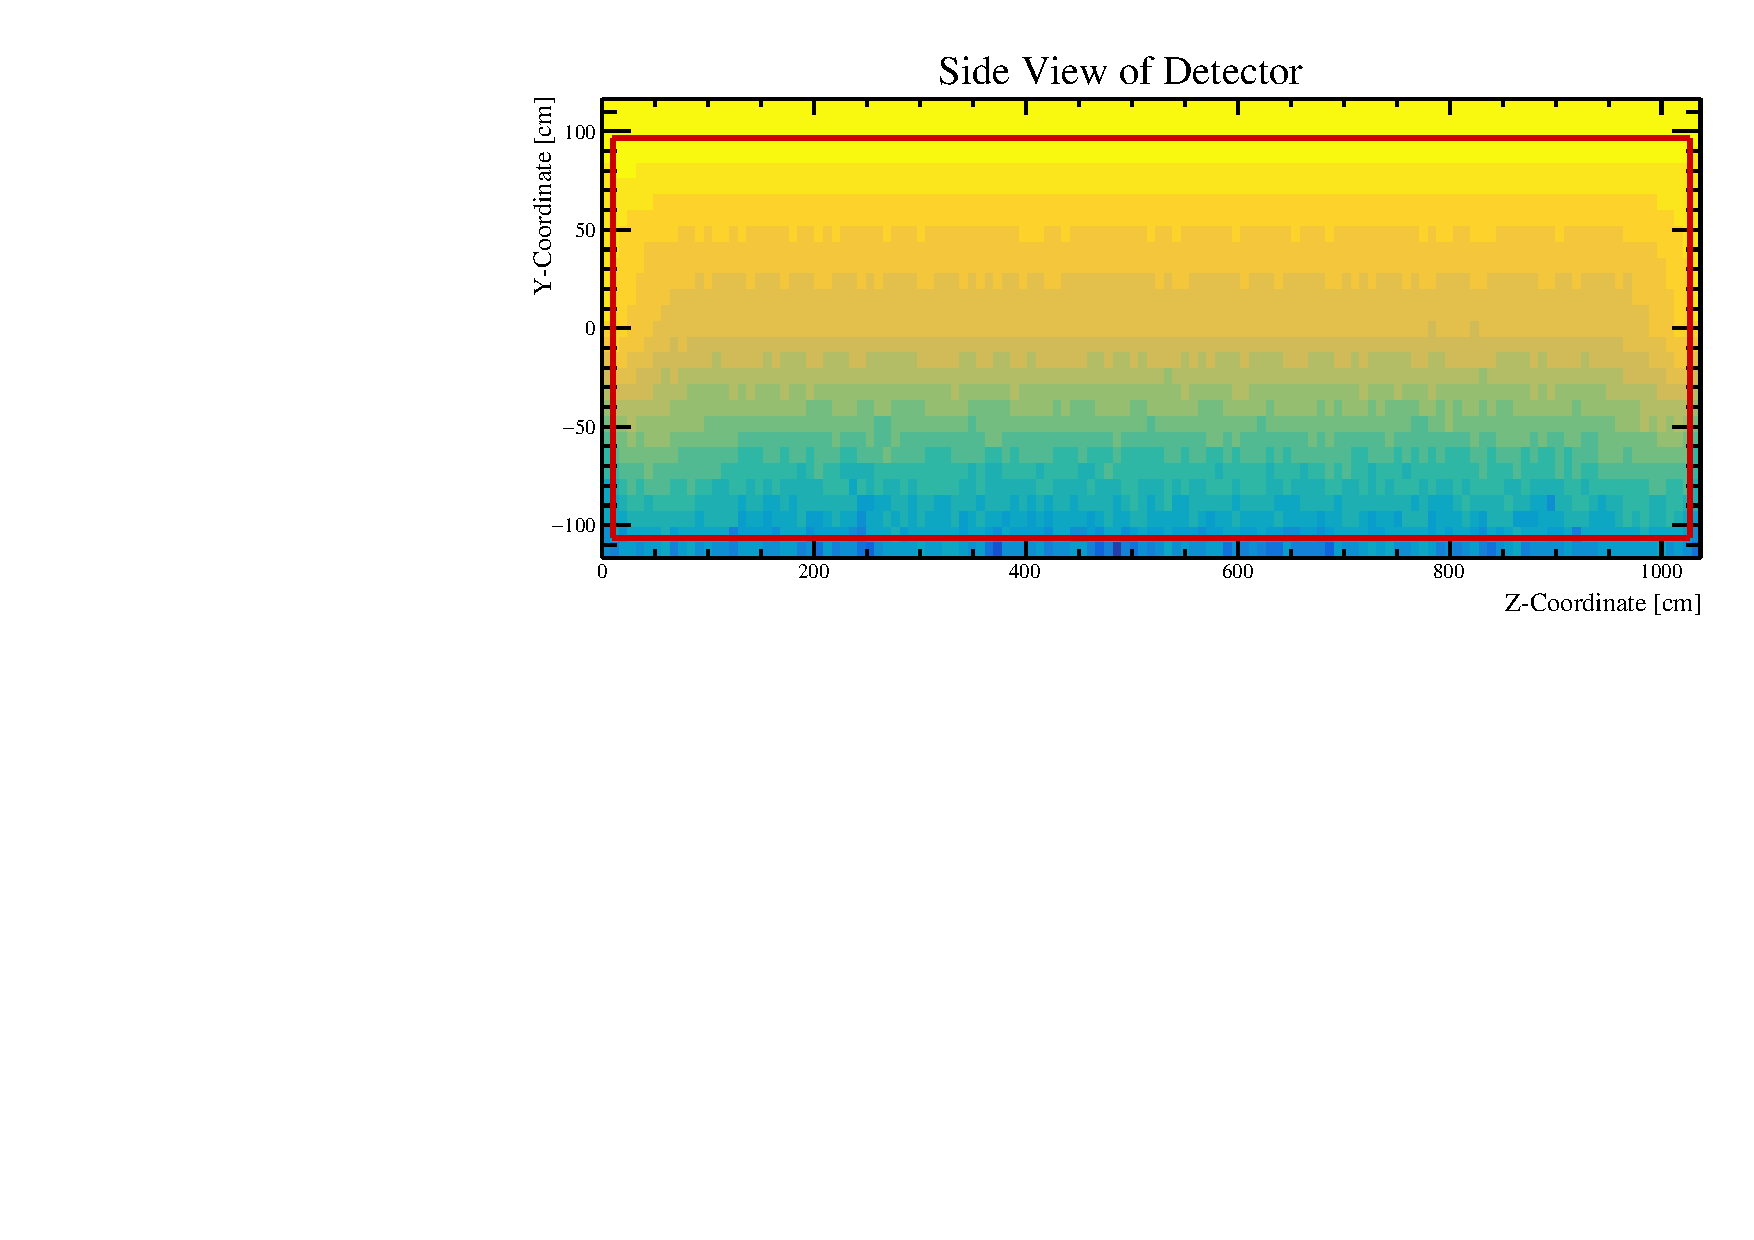
\includegraphics[height=5cm]{images/CosmicGammaBackground/SideView.pdf}
            \label{fig:GammaSideView}
        } %\qquad
        \subfloat[Background Rate Upstream View][]
        {
        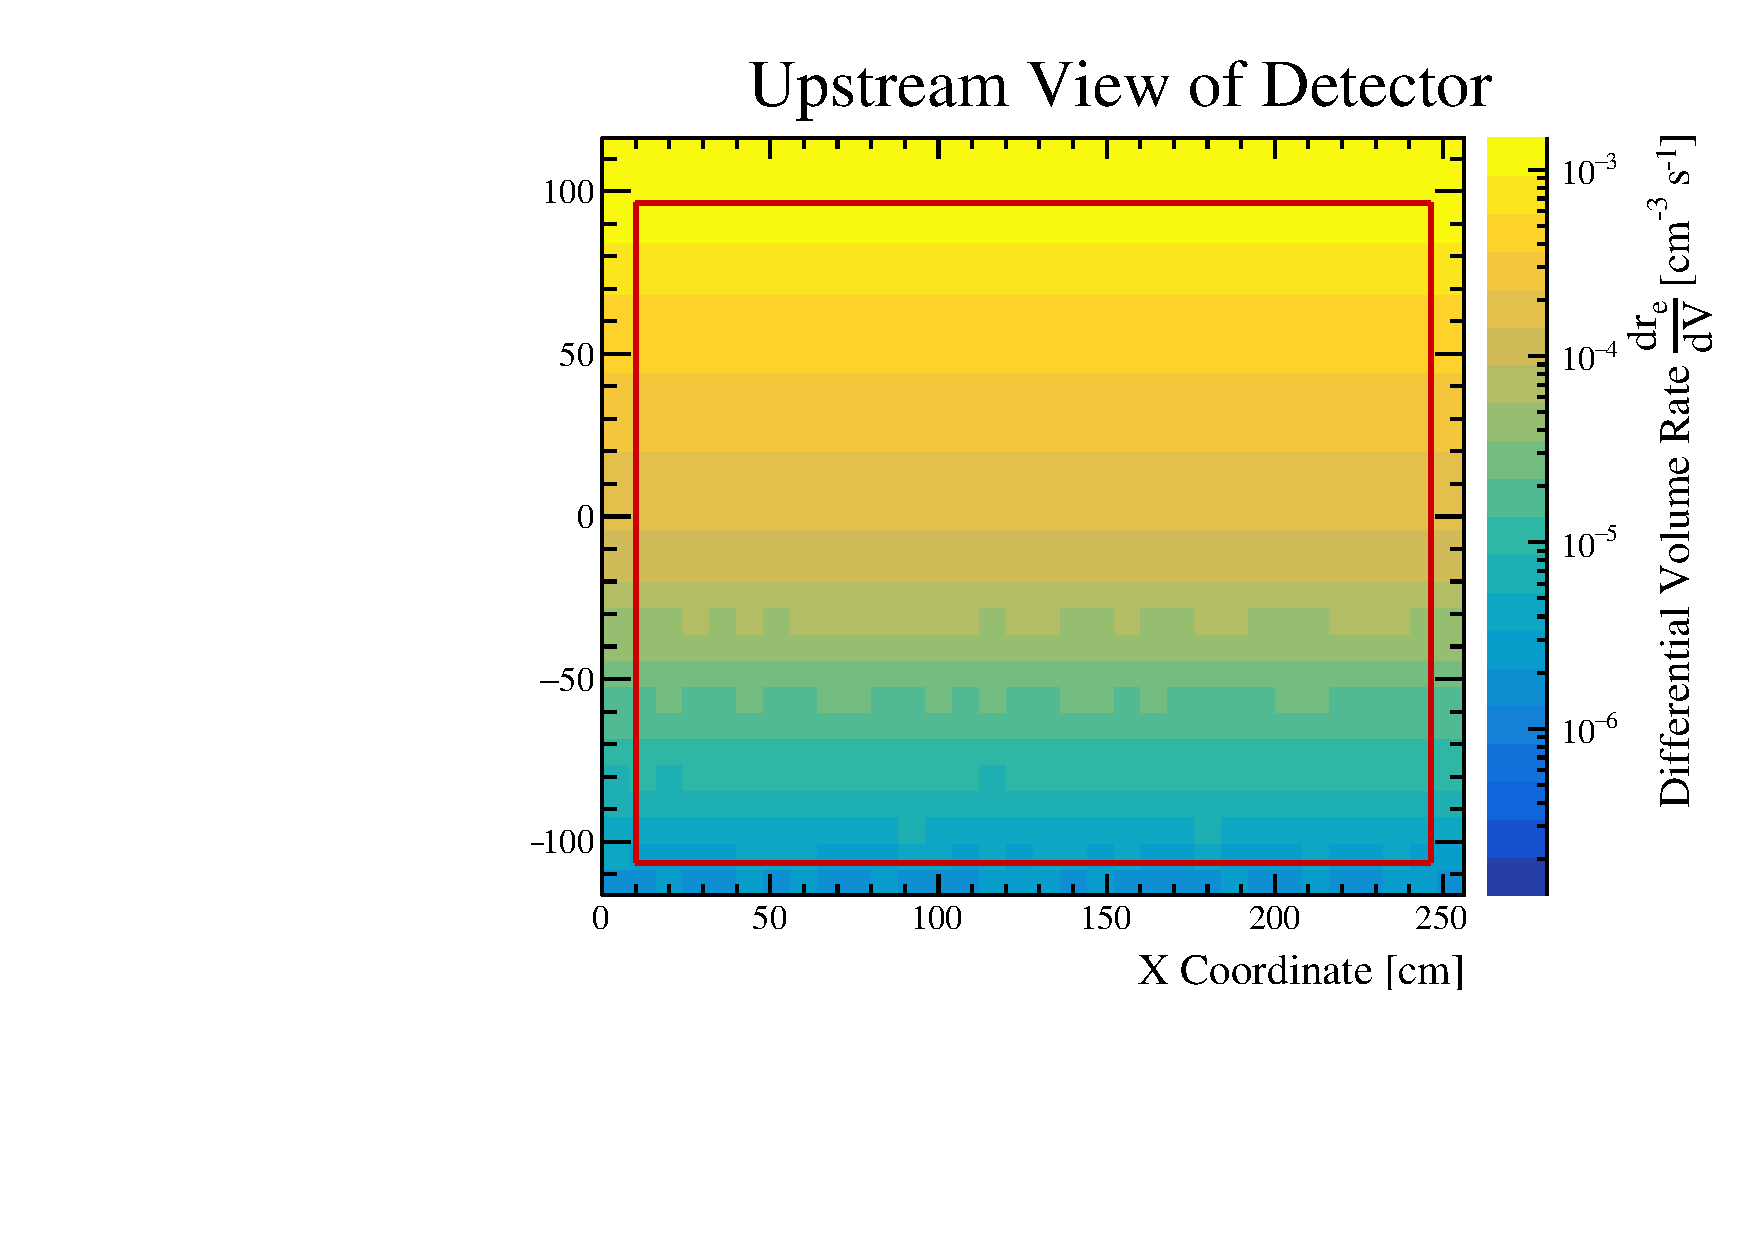
\includegraphics[height=5cm]{images/CosmicGammaBackground/UpstreamView.pdf}
            \label{fig:GammaUpstreamView}
        }
    }
    \caption[Simulated Cosmic Photon Background Rate per Volume in the MicroBooNE TPC]{These figures show simulated cosmic gamma-ray induced background rate per volume within the MicroBooNE \gls{tpc}. The background is defined as single electrons produced by cosmic gamma-rays through photoelectric effect or Compton scattering, potentially mimicking a $\nu_e$ interaction. The detector side view in \subref{fig:GammaSideView} is calculated in accordance with equation \ref{eq:BinnedDifferentialVolumeRateZY} and the upstream view in \subref{fig:GammaUpstreamView} using equation \ref{eq:BinnedDifferentialVolumeRateXY}. Furthermore, the z-coordinate of the side view is skewed by a factor of $1/2$, while the upstream view is kept at the same aspect ratio as the real detector. The red box marks the \gls{fv}, \ie every interaction occurring outside of said box will be discarded.}
    \label{fig:GammaBackgroundDistribution}
\end{figure}
As expected, the top cut appears to be the most effective, since the event rate there is more than a \num{1000} times higher compared to the one at the bottom of the \gls{tpc}. While the side cuts on the $z$-coordinate surely are cutting volumes of higher activity, the ones on the drift-axis ($x$-coordinate) do not. This can be explained by the drift-in events ensuring that the distribution stays homogenous along said axis. Still, the cut reduces the accepted volume and thus the event rate. In summary it can be said that the \gls{fv} cut is able to reduce this particular background by \SI{42.3}{\percent} (see table \ref{tab:CosmicBackgroundCuts}).

Now let us consider the angular distributions of these single electrons in the \gls{fv}, by the means of differential directional rates as introduced in equation \ref{eq:DifferentialDirectionalRate}. Analogous to equations \ref{eq:BinnedDirectionalIntensityPhi} and \ref{eq:BinnedDirectionalIntensityTheta} we can define our binned differential directional rates as,
\begin{align}\label{eq:BinnedDirectionalRatePhi}
    \frac{dr_e(\phi_n)}{d\Omega} &= \frac{\delta N_e(\phi_n)}{2T \, \delta\phi}, \\[5pt]
    \frac{dr_e(\theta_n)}{d\Omega} &= \frac{\delta N_e(\theta_n)}{2\pi T\, \delta\theta\sin{(\theta_n)}}.
    \label{eq:BinnedDirectionalRateTheta}
\end{align}
Note that the MicroBooNE coordinate system's definition of $\phi$ and $\theta$, covering a full sphere, are used instead of the azimuth $\phi^\prime$ and zenith angle $\theta^\prime$ of the standard reference system, only covering a hemisphere. This results in an additional factor of $1/2$ in $dr_e(\phi_n)d\Omega$ compared to $I_\gamma(\phi_n^\prime)$. In this case, we are interested in the \gls{2d} representation of differential angular rate as defined in equation \ref{eq:DifferentialDirectionalRate}, without any integration of the angular differentials. In binned form this results in
\begin{equation}\label{eq:BinnedDirectionalRatePhiTheta}
     \frac{dr_e(\phi_n,\theta_m)}{d\Omega} = \frac{\delta N_e(\phi_n,\theta_m)}{T\, \delta\phi \, \delta\theta \, \sin{(\theta_m)}},
\end{equation}
with the subscript $n$ denoting the bin number on the $y$-axis and $m$ the bin number on the $y$-axis of the graph shown in figure \ref{fig:FiducialAngularBackground}. On the $z$-axis, or colour axis, $dr_e(\phi_n,\theta_m)/d\Omega$ is displayed.
\begin{figure}[htbp]
    \centering
    % This operation here maxes the two plots the same height, by still providing full text width
    \subfloat[Photon Differential Directional Rate in $\phi$][]
    {
        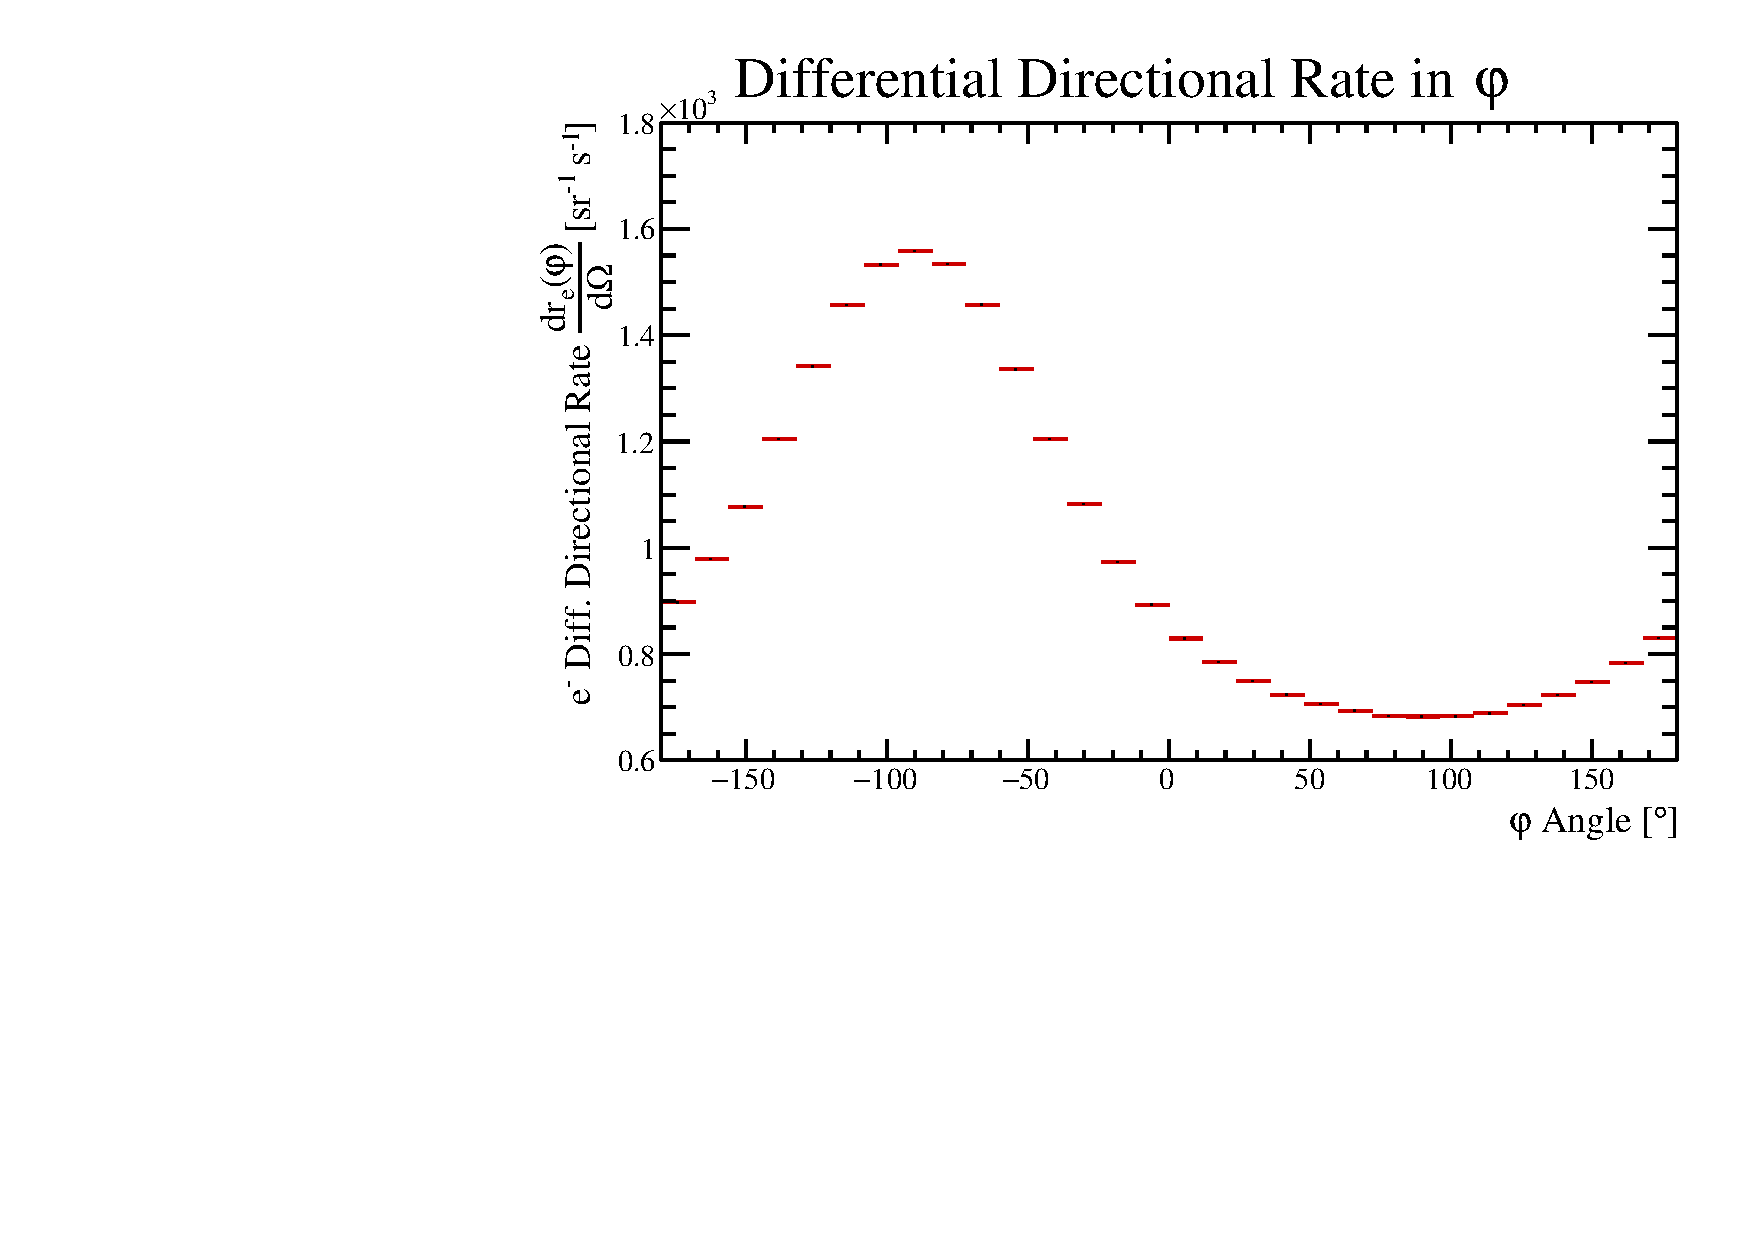
\includegraphics[width=0.48\textwidth]{images/CosmicGammaBackground/ElectronPhi.pdf}
        \label{fig:ElectronPhi}
    } %\qquad
    \subfloat[Photon Differential Directional Rate in $\theta$][]
    {
        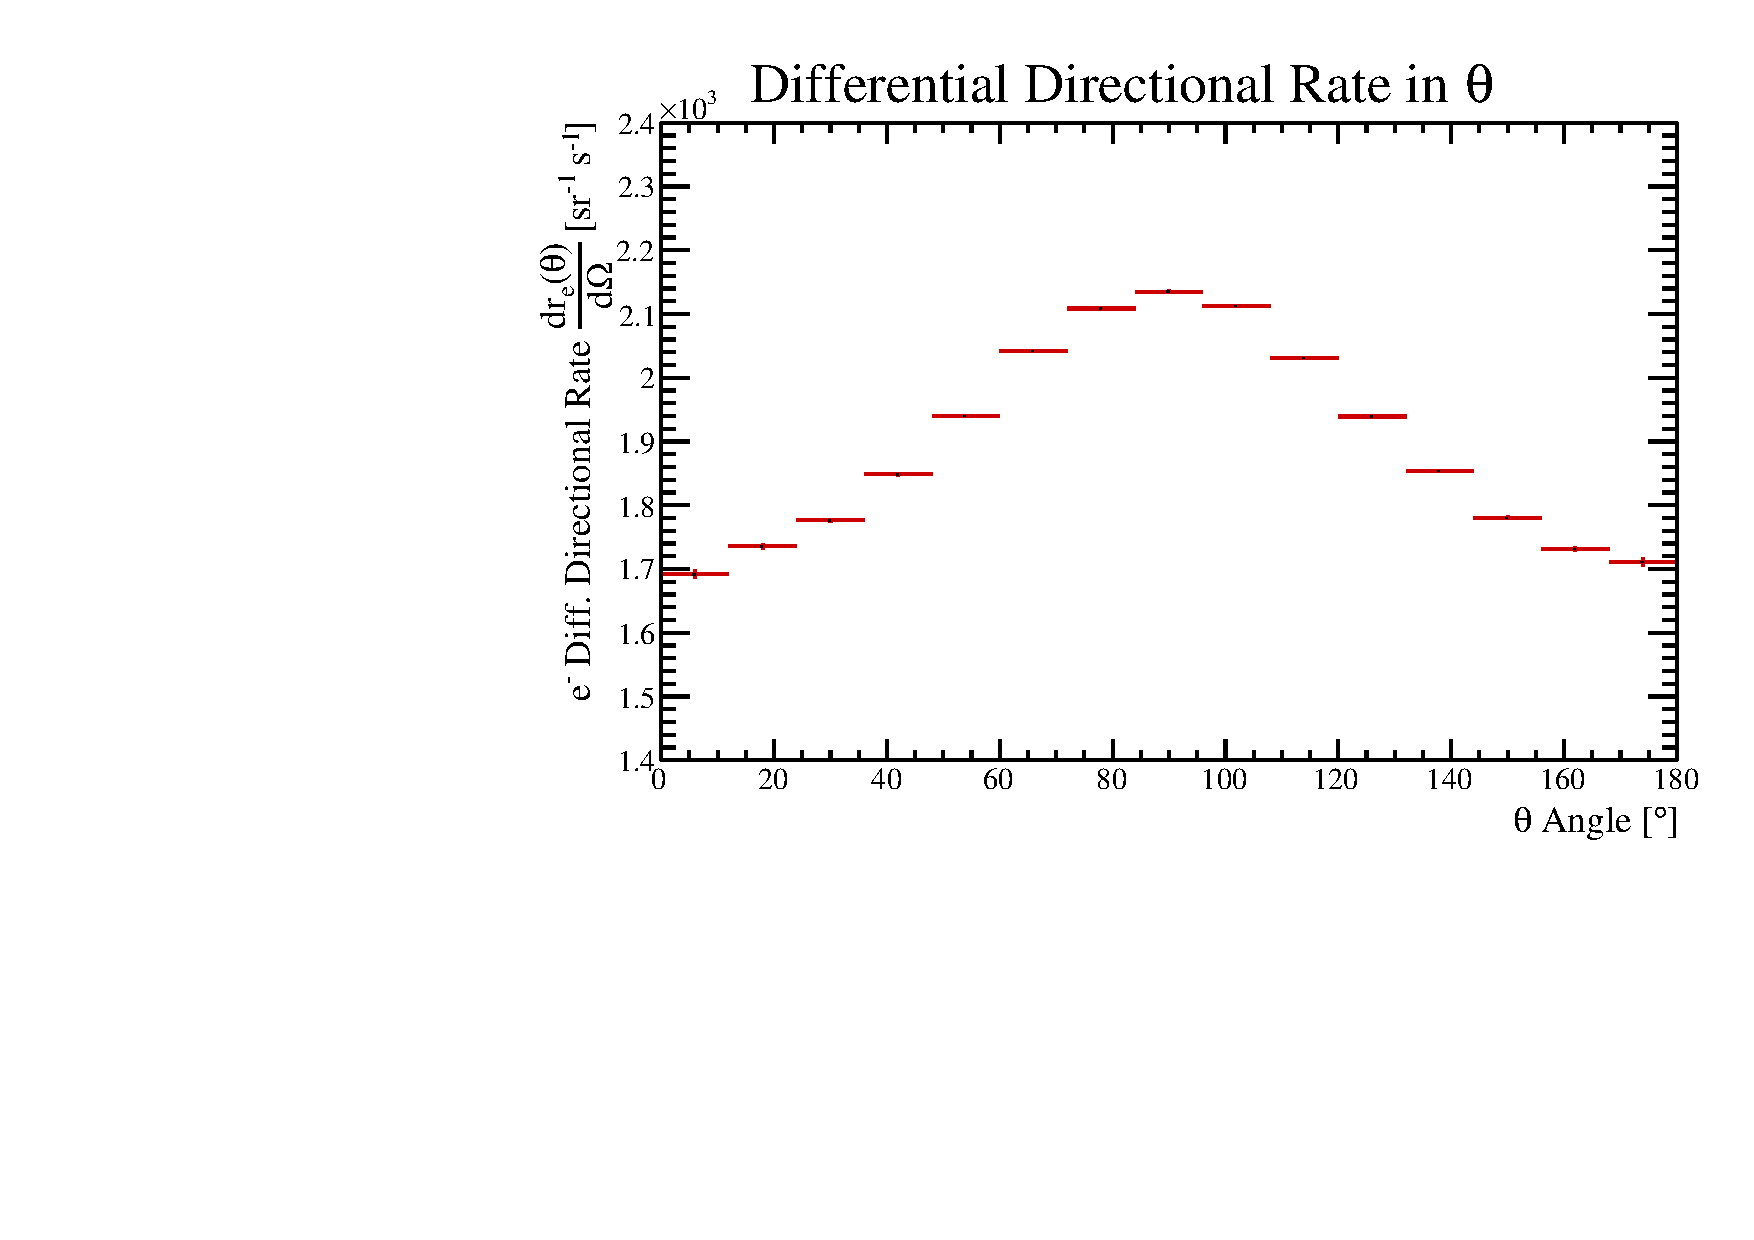
\includegraphics[width=0.48\textwidth]{images/CosmicGammaBackground/ElectronTheta.pdf}
        \label{fig:ElectronTheta}
    }
    \\
    \subfloat[Photon Differential Directional Rate in $\theta$ and $\varphi$][]
    {
        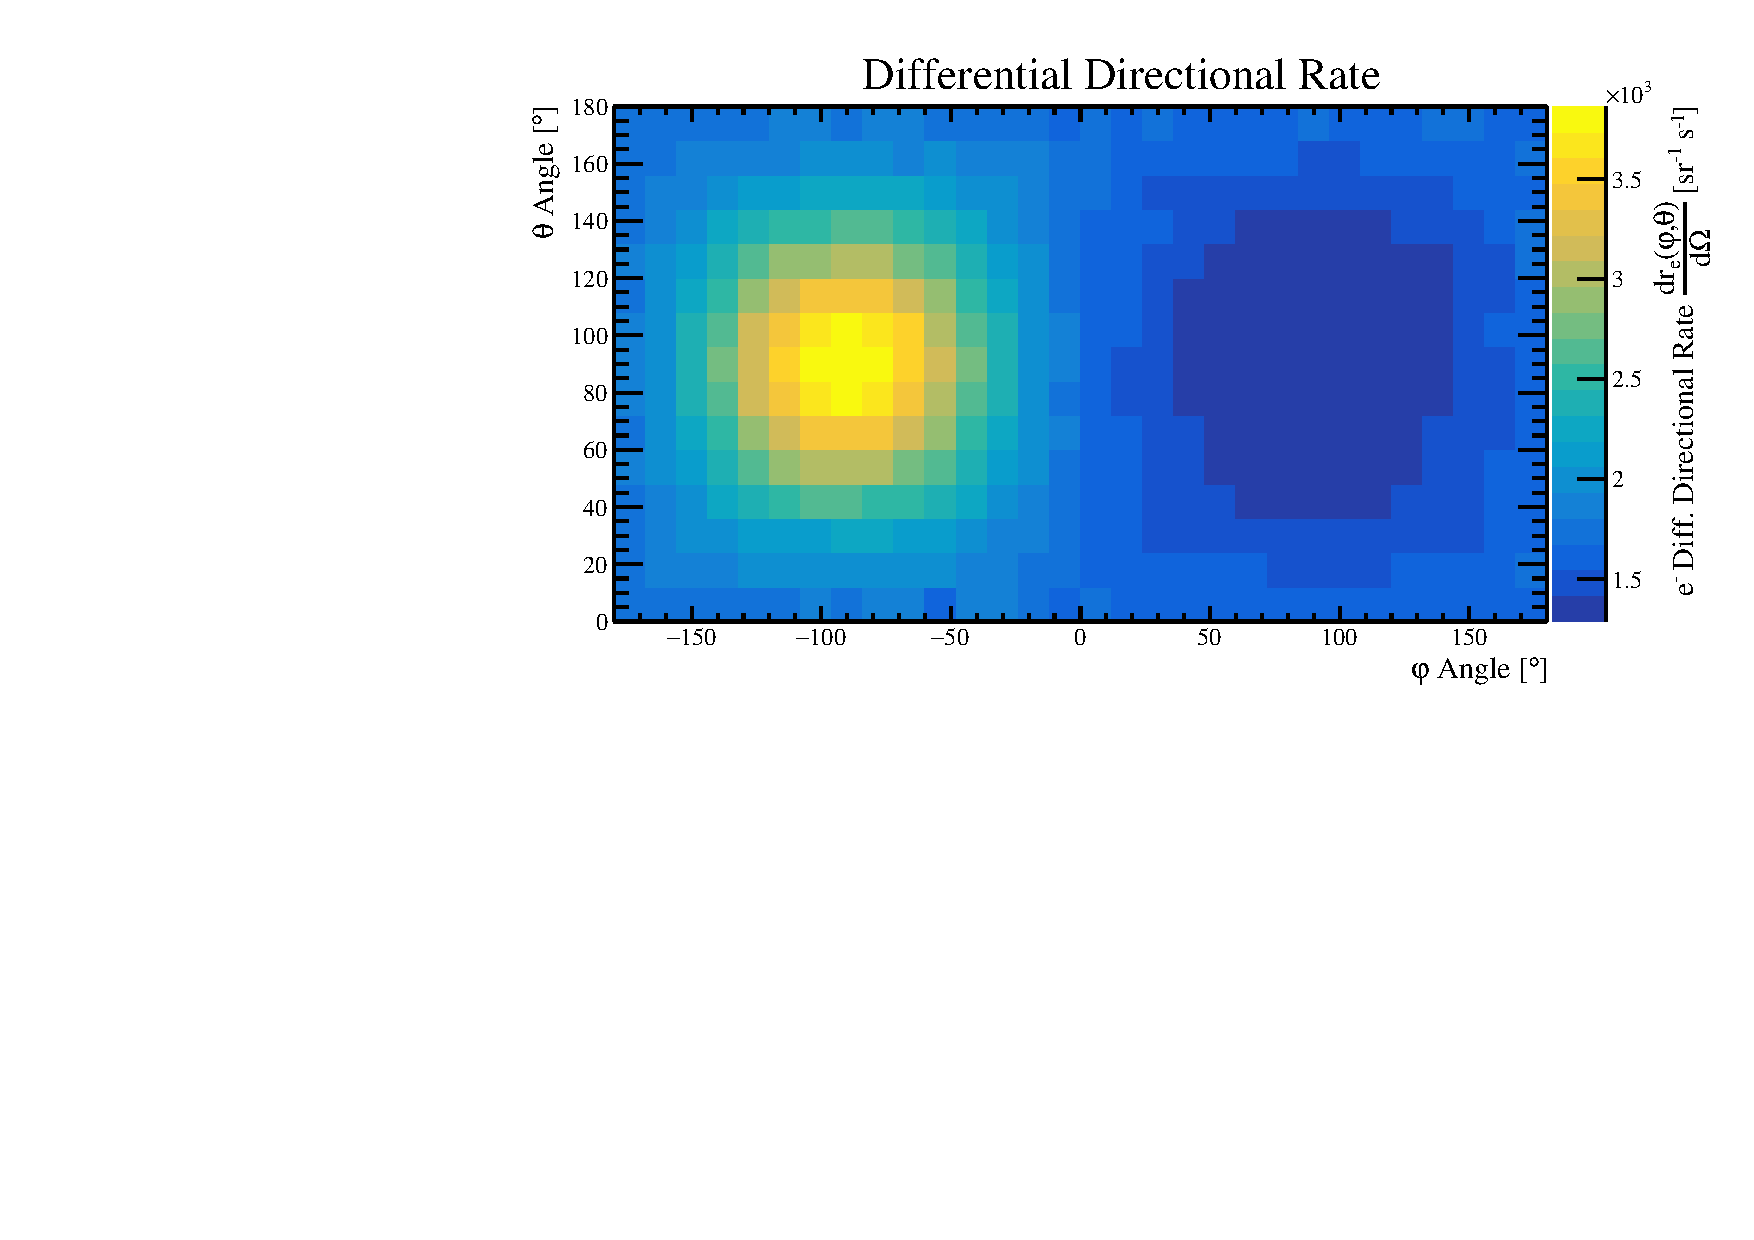
\includegraphics[width=\textwidth]{images/CosmicGammaBackground/ElectronPhiTheta.pdf}
        \label{fig:ElectronPhiTheta}
    }
    
    \caption[Differential Directional Rate Distributions of the Photon Induced Electron Background in Fiducial Volume]{These figures show the differential directional rate distributions, $dr_e/d\Omega$, of the photon induced single electron background in the \gls{fv} of the MicroBooNE \gls{tpc}. Subfigure \subref{fig:ElectronPhi} and \subref{fig:ElectronTheta} show a \gls{1d} representation of the differential directional rate, $dr_e(\phi)/d\Omega$, and $dr_e(\theta)/d\Omega$ respectively. In \subref{fig:ElectronPhiTheta} a \gls{2d} representation of said differential rate shown as a function of both angles, \ie $dr_e(\phi,\theta)/d\Omega$. To calculate the three graphs, equations \ref{eq:BinnedDirectionalRatePhi}, \ref{eq:BinnedDirectionalRateTheta}, and \ref{eq:BinnedDirectionalRatePhiTheta} are used.}
    \label{fig:FiducialAngularBackground}
\end{figure}
Examining the differential directional rates, it is becomes obvious that the main single electron background contribution is downward pointing. Down, in this case, means perpendicular to the earth's surface or the $x$-$y$-plane in the MicroBooNE coordinate system at angles $\phi = \SI{-90}{\degree}$ and $\theta = \SI{90}{\degree}$. Yet, there are plenty of electrons exhibiting shallow $\theta$ angles, below \SI{45}{\degree}, which are probably the most insidious in terms of background, since shallow $\theta$-angles are expected from electrons produced in $\nu_e$ interactions.

The next distribution I want to point out, after the \gls{fv} cut is applied, is the differential energy rate defined in equation \ref{eq:DifferentialEnergyRate}. The binned function of said equation can be derived in accordance to the binned function of the differential energy spectrum described in equation \ref{eq:BinnedDifferentialEnergySpectrum}. The differential energy rate is thus given by
\begin{equation} \label{eq:BinnedDifferentialEnergyRate}
    \frac{r_e(E_n)}{dE} = \frac{\delta N_e(E_n)}{T\, \delta E_n}.
\end{equation}
Furthermore, we can calculate the integral energy rate of the single background electrons, $R_e(E)$, defined in equation \ref{eq:IntegralEnergyRate}. Its binned function is given by
\begin{equation} \label{eq:BinnedIntegralEnergyRate}
    R_e(E_n) = \sum_{i=n}^{n_\text{max}} \frac{r_e(E_i)}{dE} \delta E_i = \frac{1}{T} \sum_{i=n}^{n_\text{max}} \delta N_e(E_i).
\end{equation}
The latter again provides the rate of electrons above a threshold energy. An essential threshold lies at $E \geq \SI{200}{\mega\electronvolt}$, because MiniBooNE observed the \gls{lee} at reconstructed neutrino energies between \SI{200}{\mega\electronvolt} and \SI{800}{\mega\electronvolt}. Hence, I would expect that the cosmic-ray photon induced single electrons would contribute substantially to the background above the \SI{200}{\mega\electronvolt} threshold in MicroBooNE. Both energy rates in the \gls{fv} are shown in figure \ref{fig:FiducialEnergyBackground} as well as the $E \geq \SI{200}{\mega\electronvolt}$ cut. 
\begin{figure}[htbp]
    \centering
    % This operation here maxes the two plots the same height, by still providing full text width
    \subfloat[Electron Background Differential Energy Rate][]
    {
        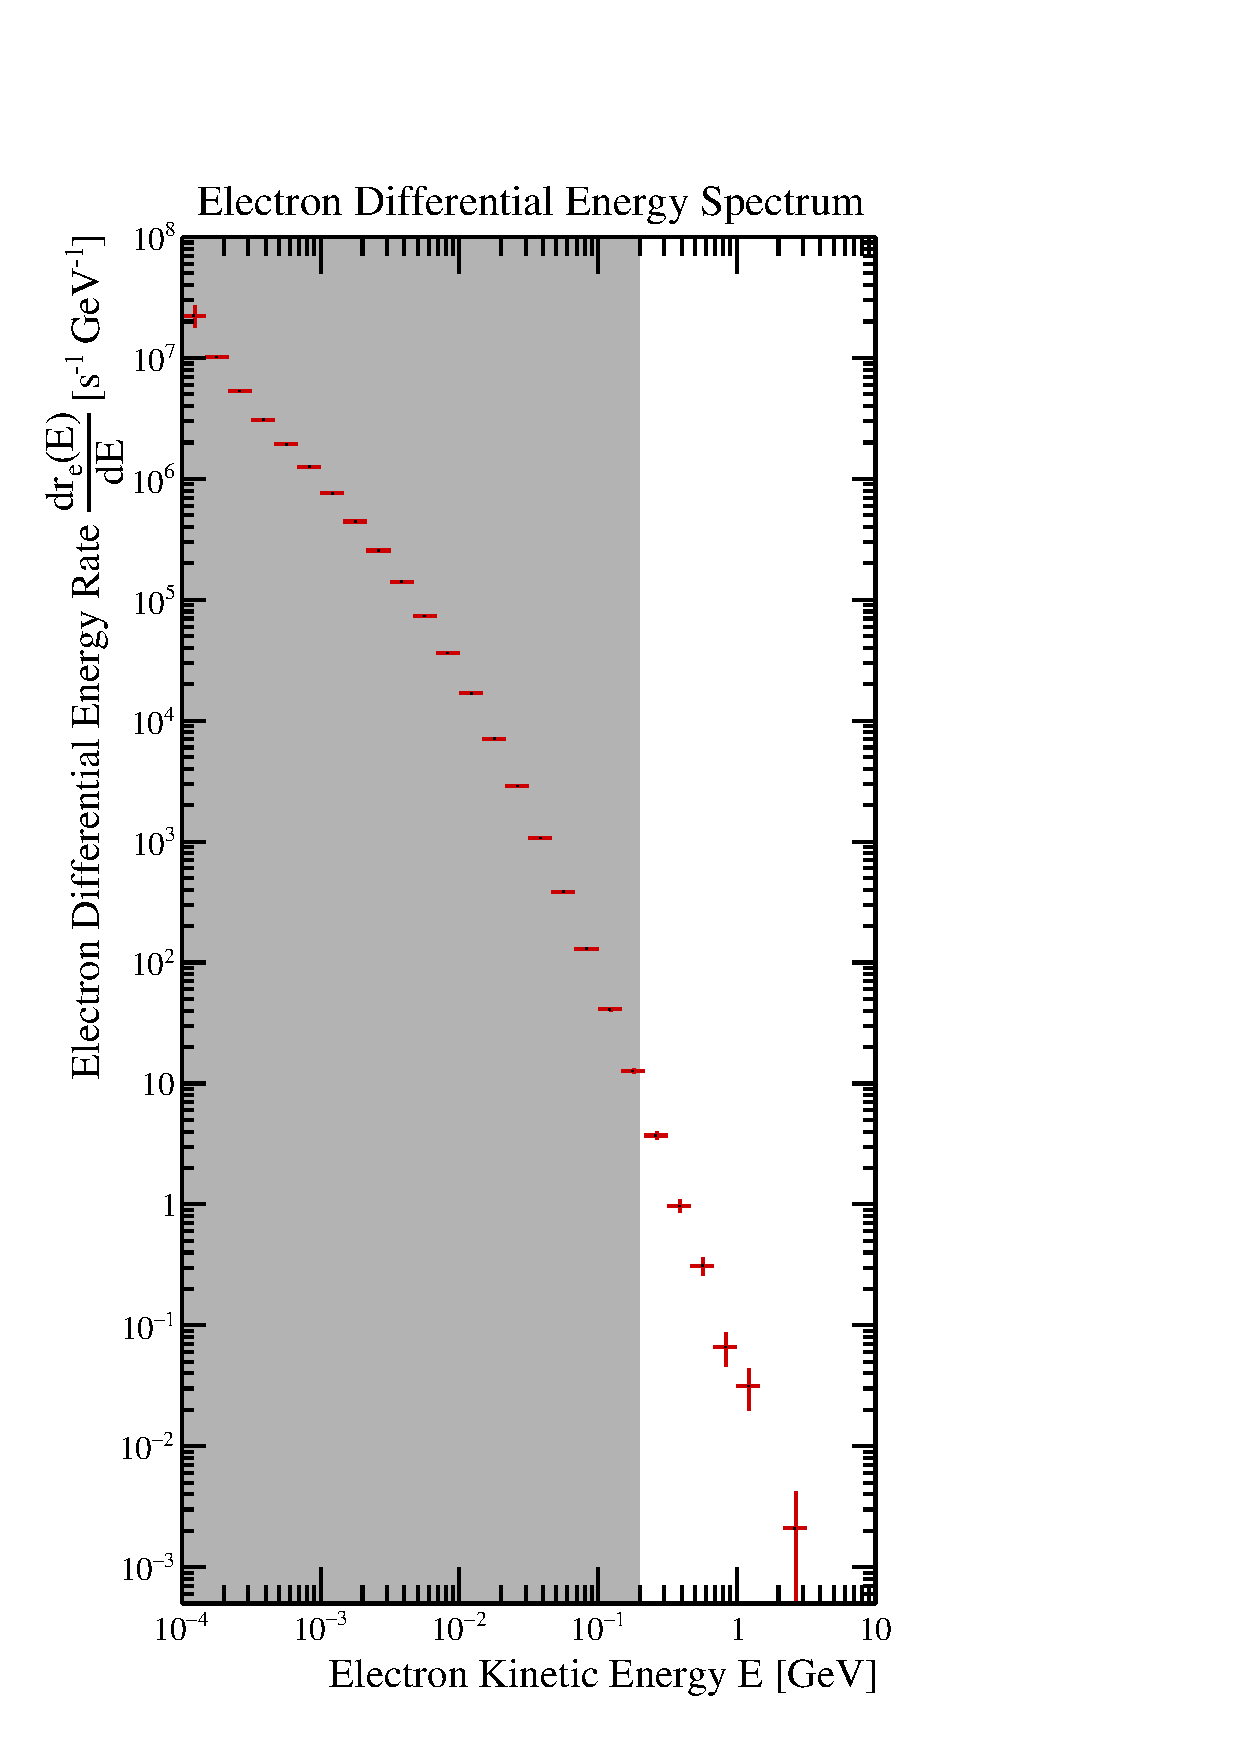
\includegraphics[width=0.48\textwidth]{images/CosmicGammaBackground/ElectronEnergy.pdf}
        \label{fig:ElectronEnergy}
    }
    \subfloat[Electron Background Integral Energy Rate][]
    {
        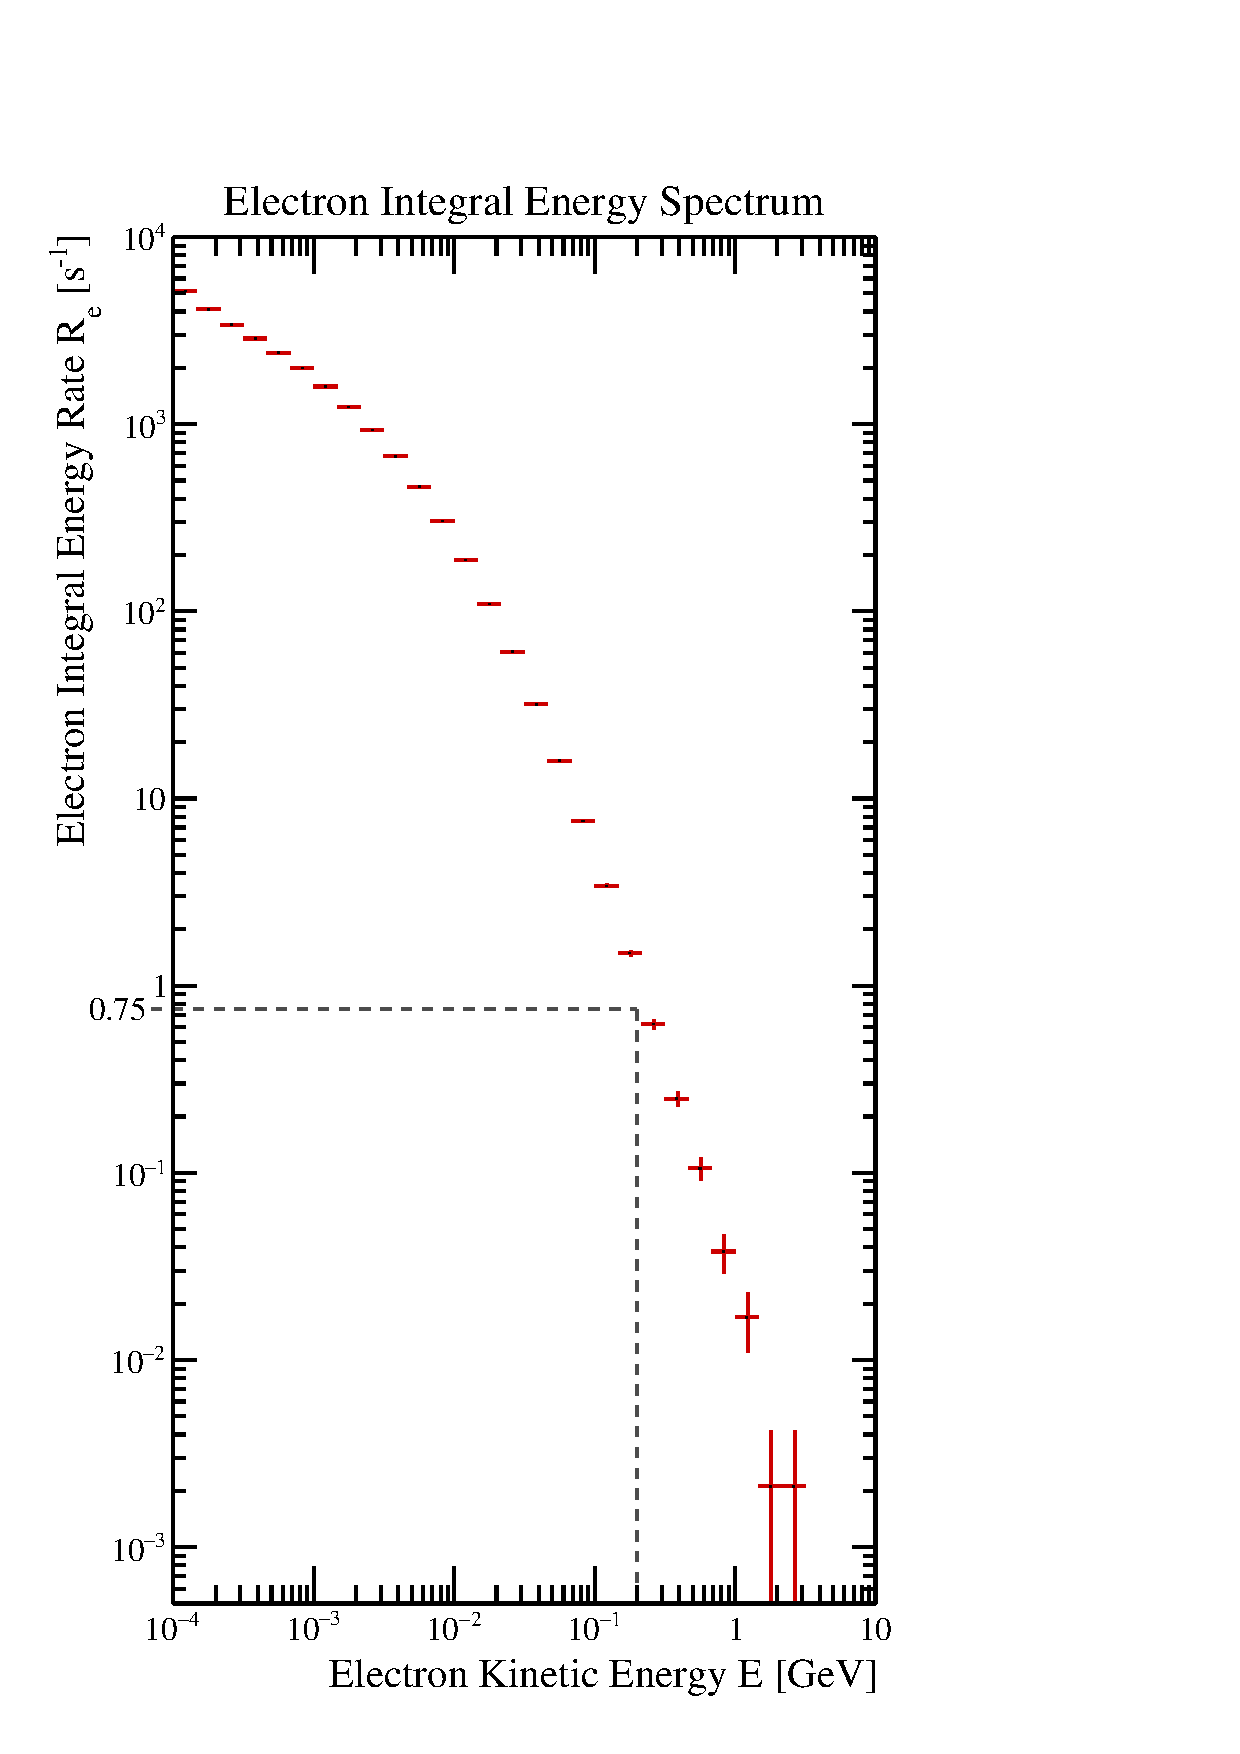
\includegraphics[width=0.48\textwidth]{images/CosmicGammaBackground/IntegratedElectronEnergy.pdf}
        \label{fig:IntegratedElectronEnergy}
    }
    \caption[Energy Distributions of the Photon Induced Electron Background in Fiducial Volume]{Depicted here are energy distributions of the photon induced electron background after applying fiducial cuts. In figure \subref{fig:ElectronEnergy} the grey area shows all energies below \SI{200}{\mega\electronvolt}, which will be cut in the next step. In \subref{fig:IntegratedElectronEnergy}, the line indicates the expected background rate of \SI{0.75}{\per\second}, when only considering electrons with $E \geq \SI{200}{\mega\electronvolt}$.}
    \label{fig:FiducialEnergyBackground}
\end{figure}
The differential energy rate, $dr_e/dE$, in figure \ref{fig:ElectronEnergy} shows similar partial power law dependence as the photon energy spectrum (see figure \ref{fig:CRYKineticEnergy}). The uptick below \SI{e-3}{\mega\electronvolt} can be attributed to the emerging dominance of the photoelectric effect in \gls{lar} (for reference see figure \ref{fig:PhotonAbsorption}). Naturally, lower electron than gamma energies are observed overall, as the photons do not loose their full energy in one single electron interaction.

As a next step I applied the aforementioned energy threshold for \gls{lee} measurements as an energy cut. With this, the usefulness of the integral energy rate can be demonstrated, as it represents the particle rate as a function of the cut energy. For $E \geq \SI{200}{\mega\electronvolt}$ the integral energy rate shows a value of $R_e(\SI{200}{\mega\electronvolt}) = \SI{0.75}{\per\second}$ or \num{1.7e-3} per readout window, which is substantial, since MicroBooNE expects a rate of $\sim\num{2e-6}$ \gls{lee} events per readout window. Consequently, the cut reduced the amount of \gls{mc} events considerably from \num{5857596} after the \gls{fv} cut to \num{357}, a reduction by \SI{99.994}{\percent}, see table \ref{tab:CosmicBackgroundCuts}. When again plotting the differential directional rate distributions, it becomes obvious, that none of the now selected high energy electrons has an upwards momentum component ($\phi > \SI{0}{\degree}$), as shown in figure \ref{fig:ECutAngularBackground}.
\begin{figure}[htbp]
    \centering
    % This operation here maxes the two plots the same height, by still providing full text width
    \subfloat[Photon Differential Directional Rate in $\phi$ with $E \geq \SI{200}{\mega\electronvolt}$][]
    {
        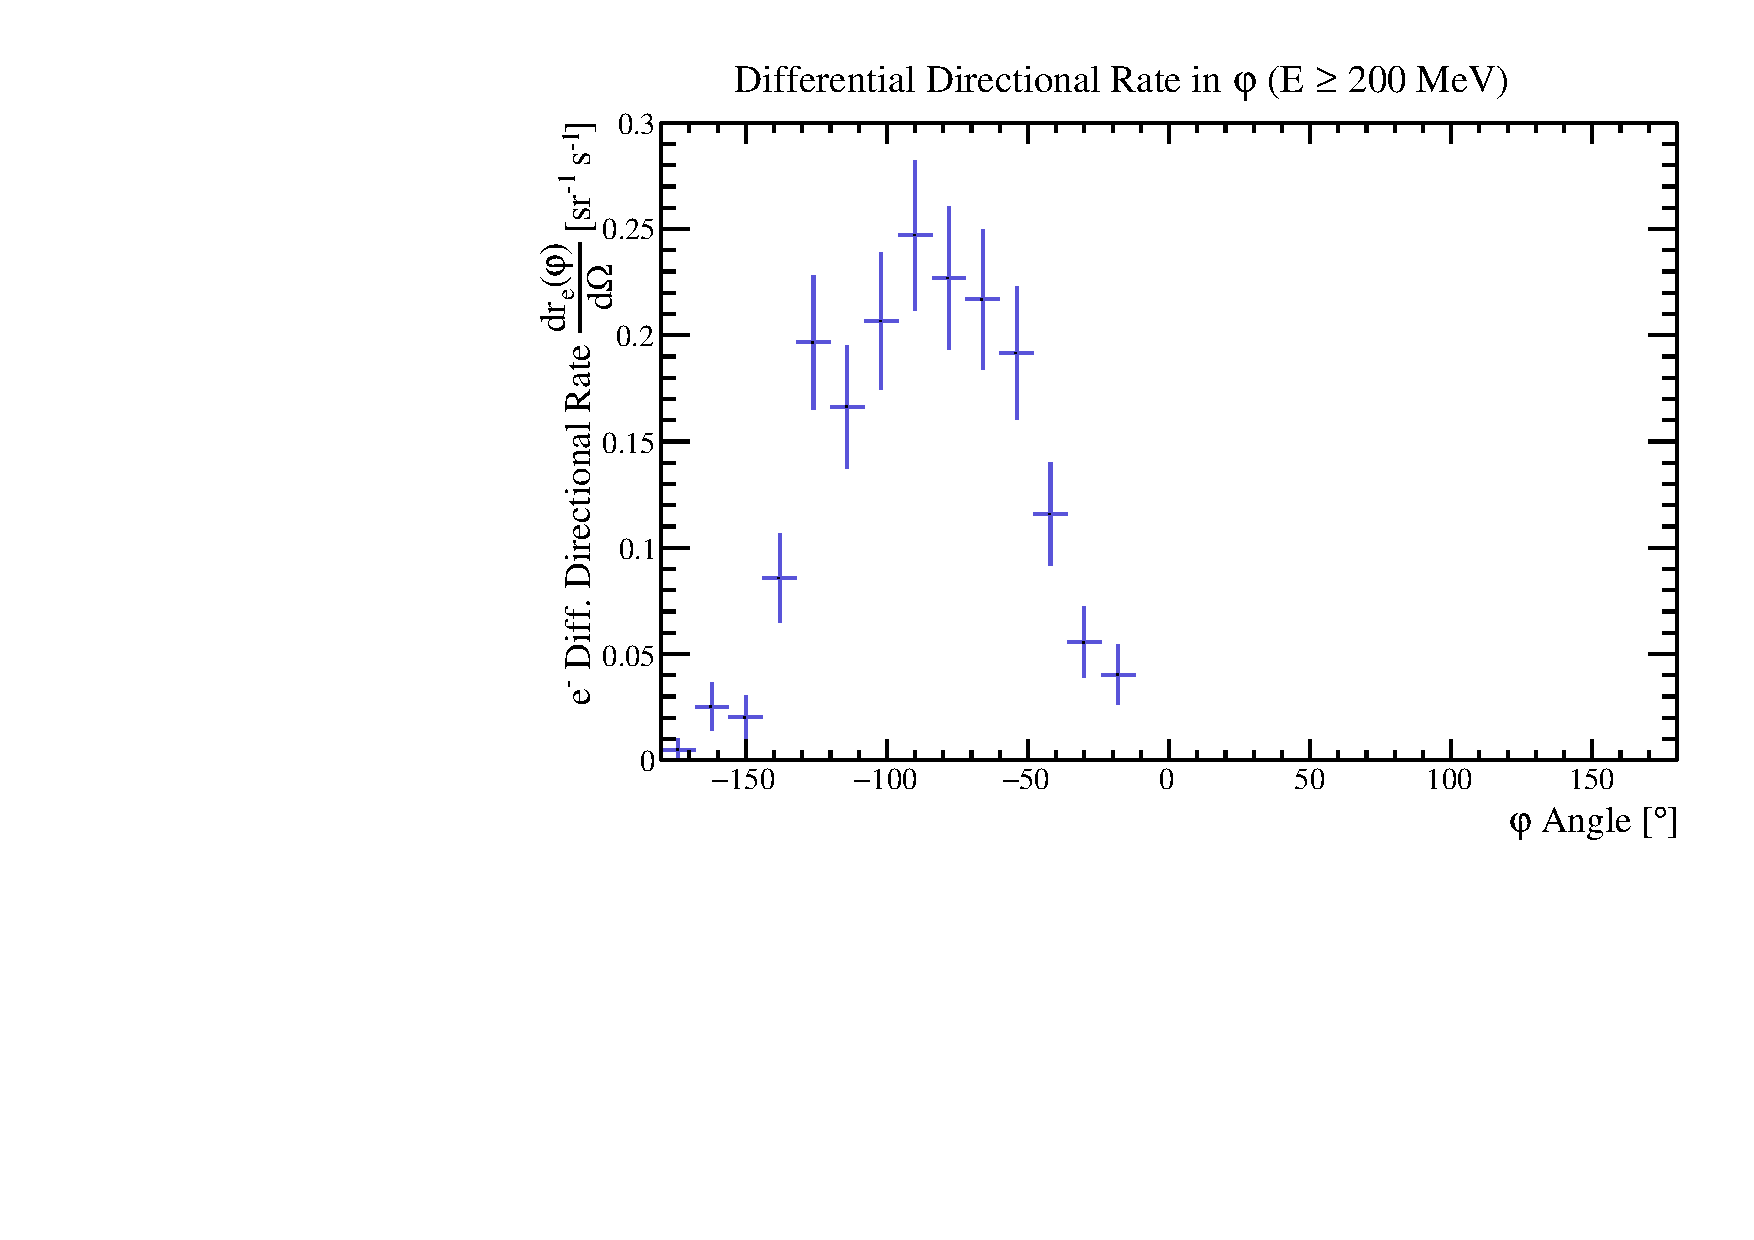
\includegraphics[width=0.48\textwidth]{images/CosmicGammaBackground/ElectronPhiECut.pdf}
        \label{fig:ElectronPhiECut}
    } %\qquad
    \subfloat[Photon Differential Directional Rate in $\theta$ with $E \geq \SI{200}{\mega\electronvolt}$][]
    {
        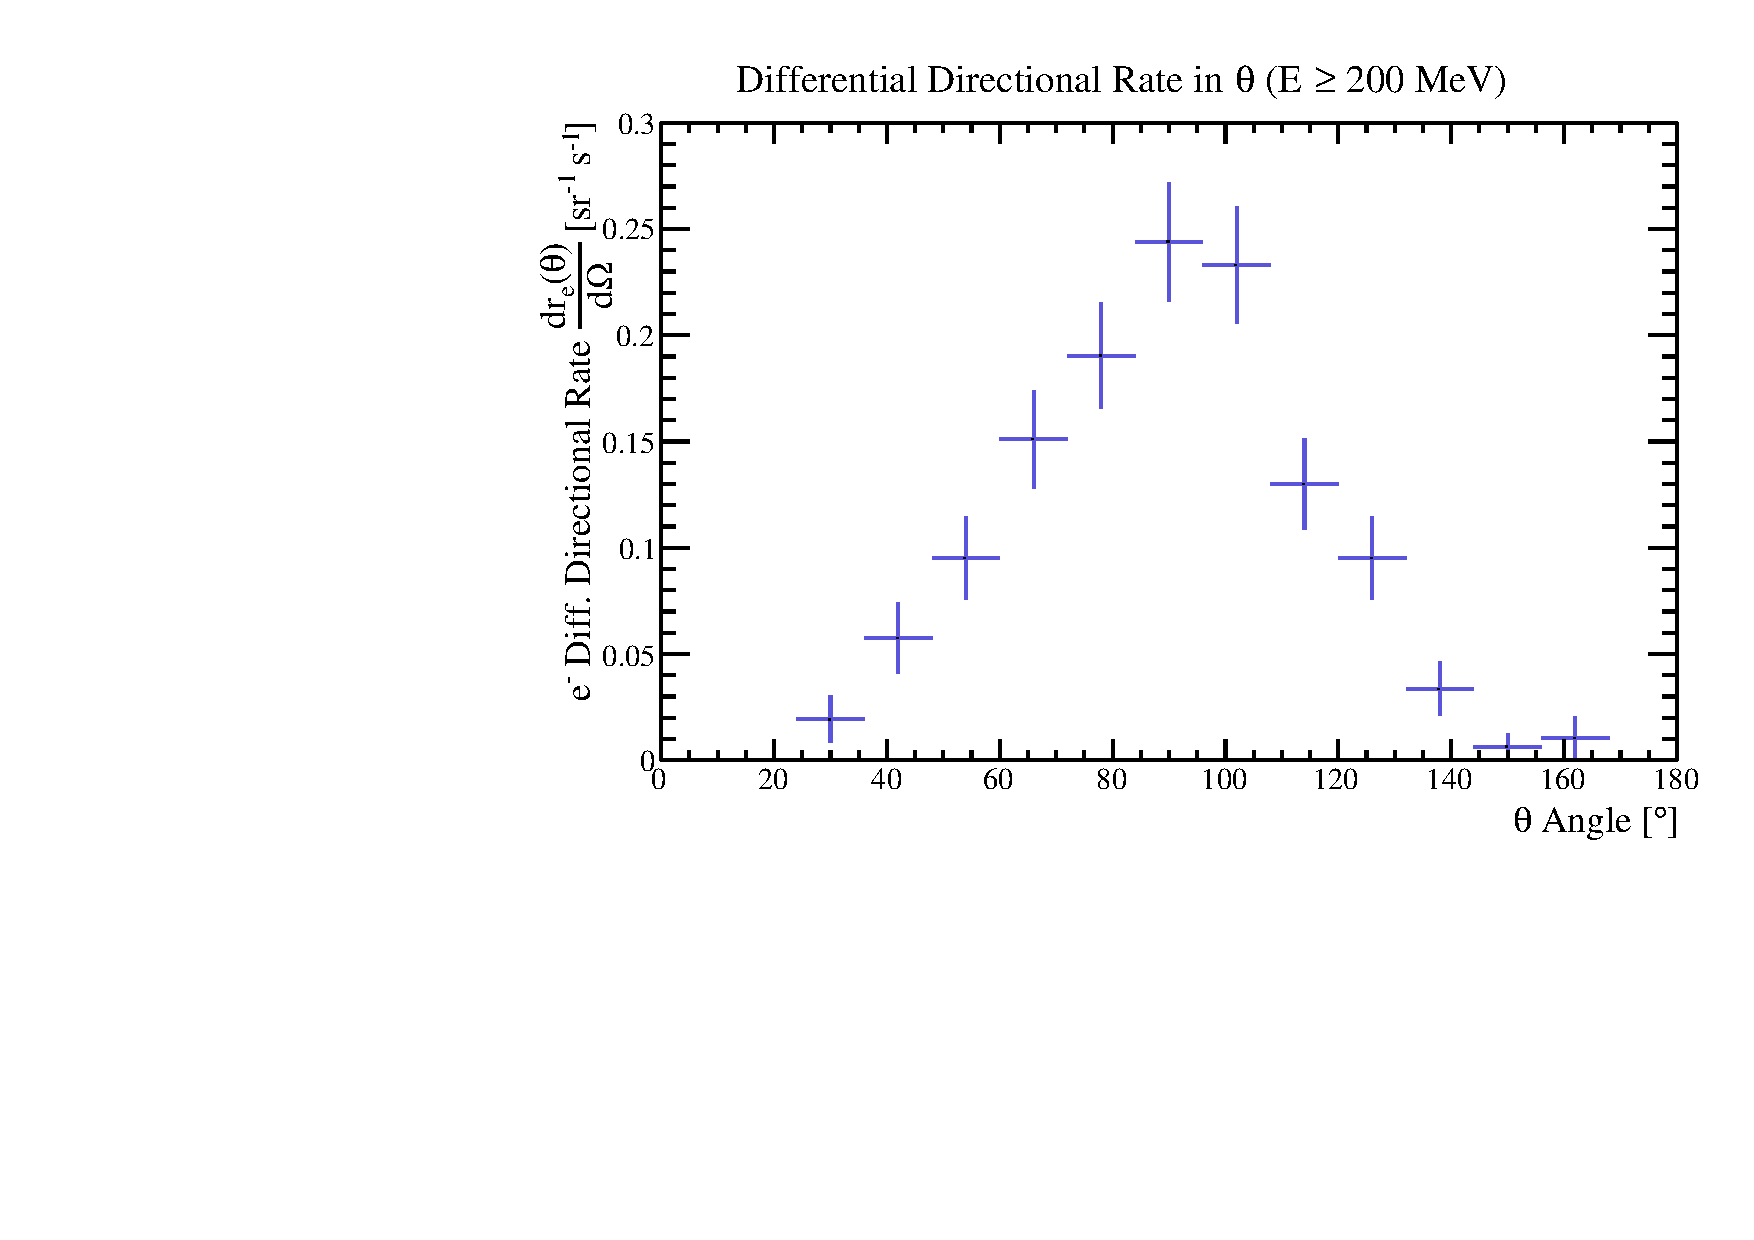
\includegraphics[width=0.48\textwidth]{images/CosmicGammaBackground/ElectronThetaECut.pdf}
        \label{fig:ElectronThetaECut}
    }
    \\
    \subfloat[Photon Differential Directional Rate in $\theta$ and $\phi$ with $E \geq \SI{200}{\mega\electronvolt}$][]
    {
        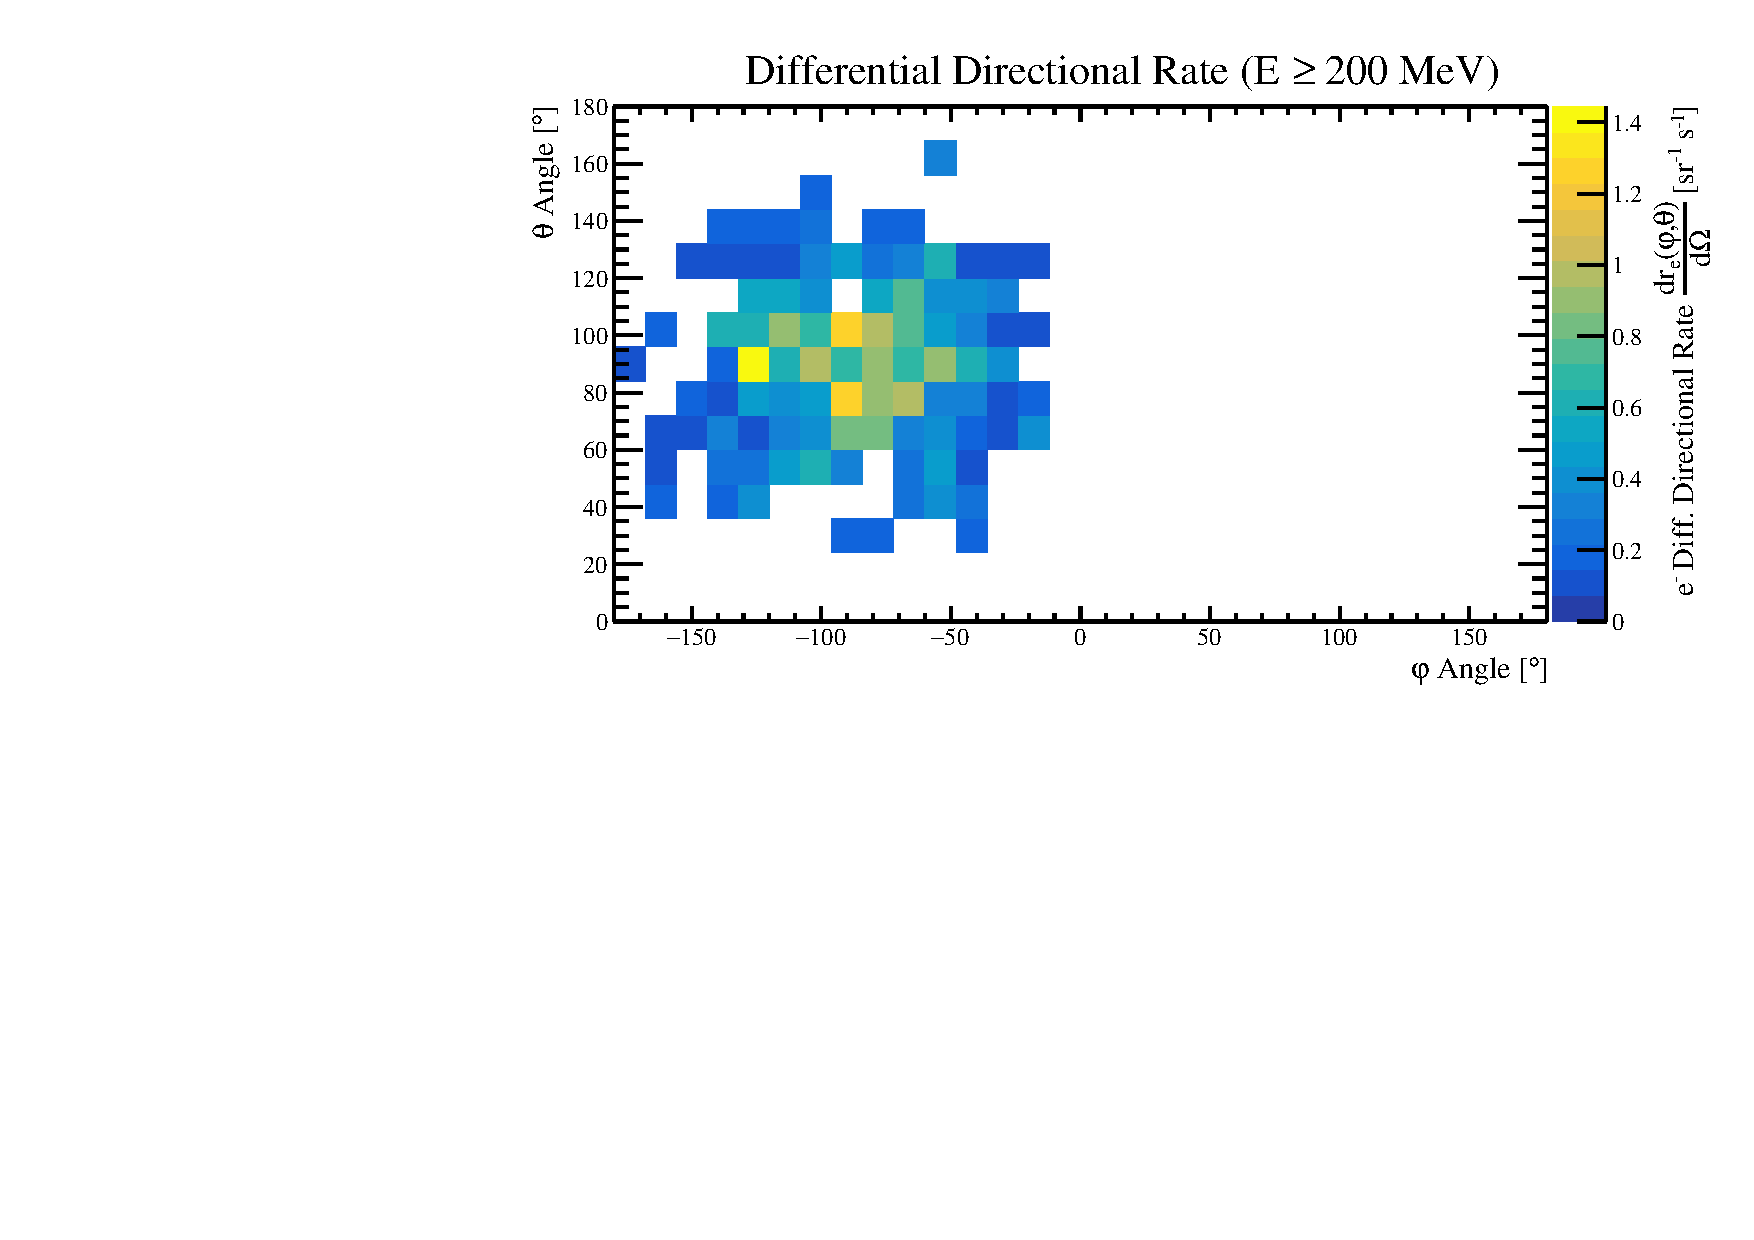
\includegraphics[width=\textwidth]{images/CosmicGammaBackground/ElectronPhiThetaECut.pdf}
        \label{fig:ElectronPhiThetaECut}
    }
    
    \caption[Differential Directional Rate Distributions of the Photon Induced Electron Background in Fiducial Volume]{The three figures show the differential directional rate distributions of the photon induced single electron background in the \gls{fv} of the MicroBooNE \gls{tpc}, with an additional energy selection of $E \geq \SI{200}{\mega\electronvolt}$. Subfigure \subref{fig:ElectronPhiECut} and \subref{fig:ElectronThetaECut} show a \gls{1d} representation of the differential directional rate, $dr_e(\phi)/d\Omega$ and $dr_e(\theta)/d\Omega$, respectively. In \subref{fig:ElectronPhiThetaECut}, a \gls{2d} representation of said differential rate is shown as a function of both angles, \ie $dr_e(\phi,\theta)/d\Omega$. The binning and the calculation methods to obtain these graphs is the same as in figure \ref{fig:FiducialAngularBackground}}
    \label{fig:ECutAngularBackground}
\end{figure}
However, there are several events with small $\theta$-angles, contributing to a possible \gls{lee} background. Any further event selection after the energy cut, is rather speculative and out of focus of this small study. Anyhow, I investigated further, although I was running low of statistics, thus the following numbers have to be viewed with a healthy dose of scepticism. When looking at electrons with $\theta \leq \SI{45}{\degree}$, for example, \num{9} events remain, which corresponds to a rate of \SI{0.019}{\per\second} or \num{4.2e-5} events per readout window of MicroBooNE. This is still \num{20} times more background than the $\sim\num{2e-6}$ \gls{lee} events per readout window MicroBooNE is looking for. A summary of all selections is listed in table \ref{tab:CosmicBackgroundCuts}.
\begin{table}[hbtp]
	\centering
    \caption[Photon Induced Background Selection Summary]{Listed here is a selection summary of the photon induced background study using ROOT. The percentage in brackets shows the survival rate of background events after each cut. Moreover, the statistical errors are only calculated for the rate per readout window, since it enhances comparability with the expected \gls{lee} signal.}
    \label{tab:CosmicBackgroundCuts}
	\begin{tabu}{lrlrr}
        \toprule
        Selection & \multicolumn{2}{c}{Number of selected $e^-$} & Rate $[\si{\per\second}]$ & per readout window \\
        \midrule
        In active volume & \num{10145342} & (\SI{100}{\percent}) & \num{21431} & \num{48.22(2)} \\
        In \gls{fv} & \num{5857596} & (\SI{57.7}{\percent}) & \num{12373} & \num{27.84(1)} \\
        $E \geq \SI{200}{\mega\electronvolt}$ & \num{357} & (\SI{0.006}{\percent}) & \num{0.75} & \num{1.7(1)e-3} \\
        $\theta \leq \SI{45}{\degree}$ & \num{9} & (\SI{1.9}{\percent}) & \num{0.019} & \num{4.2(14)e-5} \\
        \midrule
        Expected \gls{lee} & \multicolumn{2}{c}{---} & --- & $\sim\num{2e-6}$ \\ % 1.91e-6
        \bottomrule
    \end{tabu}
\end{table}

\section{Discussion of the Simulation}
It is again important to note, that this study is a rough estimate of the impact of cosmic-ray photon induced background on MicroBooNE's \gls{lee} measurement. Several assumptions were made here to simplify and thus accelerate the simulation and analysis process. These assumptions were:
\begin{enumerate}
    \item Cosmic-ray photons are the main source of single electron background.
    \item The gamma production around the active volume is in equilibrium with their absorption.
    \item The correlated cosmic showers generated by \gls{cry} are representing reality.
    \item Only single electrons are contributing to the background ($e^+$-$e^-$-pairs are eliminated).
    \item Perfect particle identification and energy reconstruction, \ie no smearing or detector effects.
    \item Only rudimentary cuts are applied in the \gls{lee} analysis.
    \item The \gls{lee} signal is not present below \SI{200}{\mega\electronvolt}, or we do not want to measure it below this threshold
\end{enumerate}
Now, let us discuss above points in more detail and rate their importance. Whether the 1\textsuperscript{st} assumption is true or not seems to be irrelevant, since it reaches beyond the scope of my analysis, specifically the investigation of the gamma induced background. I still listed it here, because other particles are able to contribute to the background, making this analysis a lower limit study. Most prominently, single electrons produced outside of the \gls{tpc} could show up as drift in events, but since electrons are mostly produced by photons anyway, this problem seems to overlap with the second assumption. The 2\textsuperscript{nd} assumption is probably the most bold one I made here. On one hand, the photons are absorbed much more efficient when entering the much denser detector environment from air. But on the other hand, spallation events and Bremsstrahlung, both photon producing processes, are also increased at the interface from air to denser materials like steel or \gls{lar}. The equilibrium assumption becomes certainly less true, the more overburden is added on top of the active volume which would result in a reduction of photon activity. Furthermore, keep in mind that the simulation assumes the detector to be at sea-level, when in reality it is located \SI{226}{\metre} \gls{asl}. Hence, the real \textbf{vertical depth} of MicroBooNE is reduced by about \SI{30}{\gram\per\centi\metre\squared} compared to the simulation. This corresponds to about \SI{21}{\centi\metre} of additional \gls{lar} overburden above the active volume. Since there is certainly a larger overburden in reality, the second assumption leads to slight overestimation of the gamma flux in the active volume. A whole section (\ref{sec:CRYAnalysis}) was dedicated to validate the 3\textsuperscript{rd} assumption and still it is hard to tell, if \gls{cry} is a reliable generator, since sea-level photon measurements are quite rare. After an in-depth analysis, I would say that \gls{cry} most probably can be trusted concerning the photon energy spectrum (see figure \ref{fig:CRYKineticEnergy}). The zenith angle distribution however, seems less reliable, especially for small angles (see figure \ref{fig:CRYDirectionalIntensityTheta}). The 4\textsuperscript{th} assumption clearly leads to an underestimation of background events, as asymmetric $e^+$-$e^-$-pairs lead to a reconstruction inefficiency and thus, to impurity in the single electron selection process. In \glspl{lartpc}, the single electron sample purity was found to be around \SI{80}{\percent} \cite{LArTPCElectronPhotonDiscrimination}, \ie about \SI{20}{\percent} of the selected single electrons were actually misidentified pair production events (see also figure \ref{fig:ElectronPhotonDiscrimination} in section \ref{sec:EnergyDissipationNeutral}). This means that my study might underestimate the event rate by up to \SI{25}{\percent}. It is, however, impossible to determine which events, at which energies are misidentified without a full detector simulation and a subsequent reconstruction. Therefore, it is non-trivial how my cuts, would influence the number of misidentified pairs. This brings us to the 5\textsuperscript{th} assumption. My simulation is, as stated above, not suited to simulate detector effects nor reconstruction effects. Since these effects simply introduce inefficiencies for all kinds of events, I do not expect them to not only impact the background in particular, but also the signal. As both would be affected the same way, the signal to background ratio stays the same at about \num{1/20}. With the 6\textsuperscript{th} assumption I tried to indicate, that I am only using rudimentary cuts which do not reflect an elaborate \gls{lee} selection. In other words: well thought out cuts could lead to great background reductions, \eg if the full $\nu_e$ momentum were to be reconstructed and a cut on the resulting $\theta$-angle were possible, the cosmic background could largely be eliminated. Concerning the 7\textsuperscript{th} assumption, the \gls{lee} measurement of MiniBooNE was limited to $E_\nu \geq \SI{200}{\mega\electronvolt}$, because of its limiting detector technology. MicroBooNE, with its superior \gls{lartpc}, is not bound to the same limit, and has much better resolution down to very low energies. Thus, the seventh assumption could be wrong. As shown in the integral energy spectrum in figure \ref{fig:IntegratedElectronEnergy}, the rate increases quite steep when decreasing the selection energy. A reduction to $E \geq \SI{100}{\mega\electronvolt}$ for example yields a background rate of \SI{3.41}{\per\second} after the energy cut, more than four times higher than with $E \geq \SI{200}{\mega\electronvolt}$. In addition the $\theta$-angles are also shallower for lower energies.

In my view, this analysis shows a good estimate of the expected single electron background and I dare say it most probably even underestimates it. With a per readout window background rate of $\sim\num{4e-5}$, my result shows that MicroBooNE is facing a challenging task with its \gls{lee} measurement, expecting a per readout window signal rate $\sim\num{2e-6}$. In principle a background is not necessarily problematic for a measurement, not even if the signal is \num{20} times smaller, as long as it can be reliably quantified. In order to deliver a reliable \gls{lee} measurement, MicroBooNE needs to either show that the cosmic-ray photon induced background can be eliminated or that it can be quantified to a high level of confidence. This study ultimately triggered the development of the \gls{crt} system at \gls{lhep} of the university of Bern, the idea being the reduction of drift in cosmic pileup events. Moreover, I was directly involved in the conception phase of the \gls{crt}, determining the dimensions of the scintillator strips used in the panels using an adapted version of the same simulation code.

% TODO Define and check readout window size (at the moment 1.6ms, it is longer though)
